\chapter{The PMT calibration in water phase}\label{sec:Introduction}
The photomultiplier tubes~(PMT) find extensive applications in the realm of particle physics, especially within neutrino experiments. A PMT is composed of a photocathode, an electron multiplier, an anode, and other essential structural components, as cited in \ref{1955Scintillation}. Photons originating from a light source and impinging upon the photocathode adhere to a Poisson process. A fraction of these photons are transformed into photoelectrons~(PE) through the photoelectric effect, and these PEs then make their way into the multiplier, as detailed in \cite{2016Optimization}. These two processes are Bernoulli selections, with the associated probabilities referred to as the quantum efficiency~(QE) and the collection efficiency~(CE). The count of photoelectrons ($n_{\mathrm{PE}}$) within a specific time interval follows a Poisson distribution, as stated in \cite{1994Absolute}.

The electron amplification is driven by the secondary electron emission~(SEE).
When an incident particle, such as electron and ion, collides with or goes through a solid surface, one or more secondary electrons are emitted~\cite{2016Secondary}.
The average number of secondaries produced per incident particle is the secondary-emission yield~(SEY, $\delta$).
The energy distribution of the secondaries~(\(\mathrm{d}\delta/\mathrm{d}E\)) is related to the energy of the incoming particle,
the incident angle, the target material, etc.~\cite{2002Probabilistic}.
Bruining and Boer~\cite{1938Secondary}, Ushio~et~al.~\cite{1988Secondary} and Jokela~et~al.~\cite{2012Secondary}
conducted target-shooting experiments using electron guns,
and measured the SEY in the current mode.
Olano and Montero~\cite{OLANO2020103456} measured the energy distribution \(\mathrm{d}\delta/\mathrm{d}E\) of Kapton, Teflon, and Ultem by charging analysis,
and found the energy of secondaries to be much smaller than that of the primary electrons.
Such results are then extrapolated to PMTs~\cite{2012An,2021Effects}.
The low light intensity at which a PMT operates makes the incident electrons discrete.
Therefore, one should be careful when extending the SEY from the current mode to a single electron case, the pulse mode.

While being amplified by the multiplier,
a single PE induces numerous electrons,
which are captured by the anode within a few hundred picoseconds.
The initial energy of the PEs produced at the photocathode is \SI{\sim 1}{eV}~\cite{Nathan1970TheED}.
The potential difference between the photocathode and the multiplier dominates the incident energy of the PEs arriving at the multiplier.
Therefore, the amplifier provides nearly identical gain for the PEs.
Because the total charge of the electrons captured by the anode is typically described by a Gaussian distribution in light of the central limit theorem of probability,
the probability density function~(PDF) of the single electron response~(SER) charge distribution is $f_{\mathcal{N}}(Q; Q_1,\sigma_1^2)$,
where $Q_1$ is the mean charge, and $\sigma_1$ is its standard deviation.
The PE count $n_{\mathrm{PE}}$ follows a Poisson distribution with the probability mass function $P_\pi(n_{\mathrm{PE}};\lambda)$,
where $\lambda$ is the expected PE count at a certain light intensity.
After amplification, the total charge distribution $f(Q)$ is a folding of the Poisson distribution and the SER charge distribution~\cite{1994Absolute}.
There are two types of background processes.
The first one follows a low-charged finite-width Gaussian~$\mathcal{N}(0,\sigma_0^2)$ without any PEs emitted from the photocathode.
The second process is discrete with a probability $w$.
Examples include thermoemission and noise generated by incident light.
This discrete process follows an exponential distribution~$\mathrm{Exp}(\alpha)$,
with $\alpha$ being the rate of exponential decay.
Considering the charge distribution of the two types of background processes being $f_{\mathrm{b}}(Q)$,
the overall charge distribution can be expressed in Eq.~(\ref{eq:sreal}):
\begin{equation}
	\begin{aligned}
		f(Q) =  & P_{\pi}(n_{\mathrm{PE}}=0;\lambda)f_{\mathrm{b}}(Q) + \sum_{n_{\mathrm{PE}}=1}^{\infty}P_{\pi}(n_{\mathrm{PE}};\lambda) f_{\mathcal{N}}(Q; n_{\mathrm{PE}}Q_1,n_{\mathrm{PE}}\sigma_1^2) \\
		\approx & \left\{\frac{(1-w)}{\sigma_0 \sqrt{2 \pi}} \exp \left(-\frac{Q^2}{2 \sigma_0^2}\right)
		+w \theta(Q)\times \alpha \exp \left(-\alpha Q\right)\right\} \mathrm{e}^{-\lambda}                                                                                                                \\
		        & +\sum_{n_{\mathrm{PE}}=1}^{\infty} \frac{\lambda^{n_{\mathrm{PE}}} \mathrm{e}^{-\lambda}}{n_{\mathrm{PE}} !}
		\times \frac{1}{\sigma_1 \sqrt{2 \pi n_{\mathrm{PE}}}}\times
		\exp \left(-\frac{\left(Q-n_{\mathrm{PE}} Q_1\right)^2}{2 n_{\mathrm{PE}} \sigma_1^2}\right)
	\end{aligned}
	\label{eq:sreal}
\end{equation}
where $\theta(Q)$ is the Heaviside function.
When $\lambda$ is less than 0.1,
the probability of observing two or more PEs is less than one-tenth of the probability of observing a single PE.
In this case, the charge distribution will only show the peak of the pedestal~($Q=0$) and the peak of the single PE~($Q=Q_1$) as indicated in the blue histogram in Fig~\ref{fig:spe_sreal}.
We can obtain an approximate SER charge spectrum after applying some cuts to remove the pedestal.
Our work aligns different PMTs' gain by dividing the SER charge spectrum with $Q_1$ as $Q/Q_1$.

\section{The single electron response of MCP-PMTs}
\subsubsection{The newly developed MCP-PMT}
Instead of a large-sized dynode-chain commonly used in PMTs,
MCP-PMTs employ MCPs as electron multipliers.
MCP-PMTs are currently in use or planned for neutrino experiments
like the JUNO~\cite{ZHU2020162002} and the Jinping Neutrino Experiment~\cite{Zhang:2023ued},
collider experiments like the Belle II TOP detector~\cite{MATSUOKA2014148} and the PANDA DIRC Cherenkov detector at FAIR~\cite{KRAUSS2023168659},
and cosmic ray observatories like the Large High Altitude Air Shower Observatory~\cite{Cao2019UpgradingPT}.
Initially, the fact that the feedback ions cause damage to the photocathode
led to a lifetime issue of MCP-PMTs~\cite{N2006Lifetime}.

The atomic layer deposition~(ALD) technique~\cite{2012An}
is applied to fabricate MCP-PMTs solving the lifetime issue~\cite{Lehmann:2022ret}.
Chen~et~al.~\cite{2016Optimization} indicated that depositing high SEY materials
such as \ce{Al2O3} via ALD on the input electrode of the first MCP
can enhance the probability of collecting the secondaries to improve CE
to nearly \SI{100}{\%} rather than being constrained by the MCP open-area ratio.
This enhancement is later extended to a composite \ce{Al2O3}-\ce{MgO} layer
by Cao~et~al.~\cite{cao_secondary_2021} and Zhang~et~al.~\cite{zzj2021Al}
to allow for increased gain, improved single electron resolution,
and a higher peak-to-valley ratio of the MCP-PMTs~\cite{2021Effects}.

In the performance tests to evaluate the 8-inch high-CE MCP-PMT by the Jinping Neutrino Experiment,
\emph{jumbo charges} are found in the SER charge spectra~\cite{Zhang:2023ued},
as shown in the red histogram in Fig~\ref{fig:spe_sreal}.
Similar charges have also been observed in the mass testing of the 20-inch MCP-PMTs at JUNO,
identified as the ``long tail'' in the SER charge distribution~\cite{JUNO:2022hlz}.
Orlov~et~al.~\cite{reviewer1} reported that the pulse height distribution of the high-CE MCP-PMTs had a non-Gaussian long-tail structure.
Zhang~et~al.~\cite{2021Gain} used the charge model in Eq.~\eqref{eq:sreal} for the jumbo charges and recommended an extra gain calibration.
Yang~et~al.~\cite{2017MCP} conducted a voltage-division experiment to reveal that the MCP gain for the low-energy electrons is significantly smaller than
that for the high-energy ones.
Thus, the MCP gain for the secondaries differs from that for the PEs entering the channels directly.
The SER charge model in Eq.~\eqref{eq:sreal} is no longer sufficient to accurately calibrate this type of PMT.
Understanding the origin of the jumbo charges is necessary for an appropriate SER charge calibration.

\begin{figure}[!htbp]
	\centering
	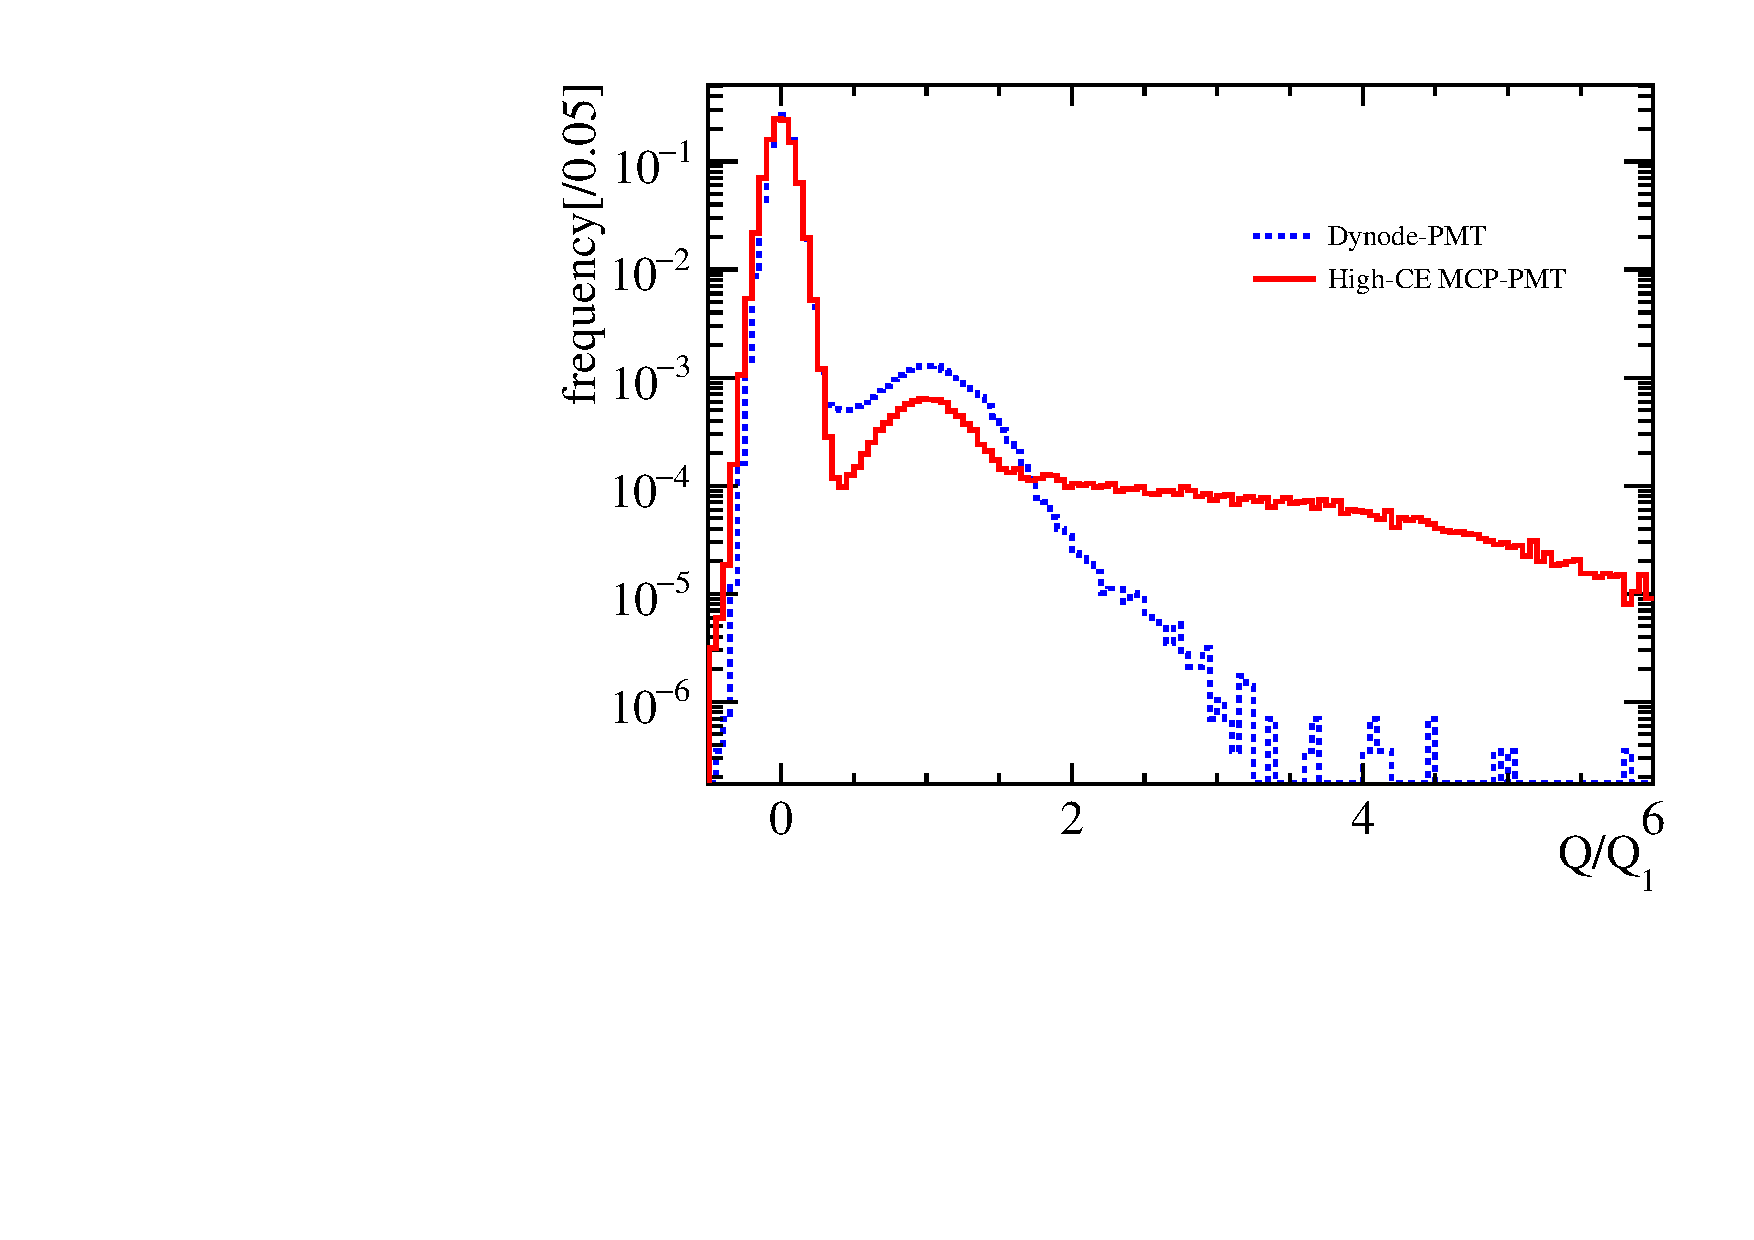
\includegraphics[width=0.5\textwidth]{PMTRelated/GTmodel/spe.pdf}
	\caption{The charge spectrum of the high-CE MCP-PMT GDB-6082~(red) and a dynode-PMT~(blue)~\cite{Zhang:2023ued}.
		The blue histogram consists of the pedestal $Q=0$ and the principal peak of $Q=Q_1$, while the red histogram includes jumbo charges.}
	\label{fig:spe_sreal}
\end{figure}

To elucidate the nature of the jumbo charges, the Gamma distribution is introduced and a voltage-division experiment is developed to measure the relationship
between MCP gain and the energy of the incident electrons.
Considering the SEE model, we elucidate the nature of the jumbo charges
and calculate the total SEY of the \ce{Al2O3}-\ce{MgO} layer when the incident energy is \SI{650}{eV}.
Through convolution-based modeling, the physical mechanisms driving have been clarified, and a quantitative mathematical framework establishe, which is the first formulation for these kind of high-CE MCP-PMTs.

\subsection{Gamma-Distributed SER charges}\label{gammapossion}
Every multiplication of electrons at the dynodes or MCP channels follows approximately a Poisson distribution~\cite{branchandPoisson}.
A series of such multiplications forms cascaded Poissonians~\cite{1955Scintillation} and is
an example of the branching process~\cite{Bartlett1963TheTO} challenging to perform analytical computations.
Woodward~\cite{Woodward} argued that the SER charge spectrum exhibits an intermediate shape between a Poisson and a Gaussian.
Prescott~\cite{polya} proposed a cascaded Polya distribution to characterize the electron multiplication in PMT,
particularly when considering the non-uniformity of the dynode surface.
Kalousis~\cite{2012Calibration,2020A} approximated the Polya distribution as a Gamma one to calibrate PMT
and achieved better results than the Gaussian model in Eq.~\eqref{eq:sreal}.

Instead of the Gaussian containing a small nonphysical tail less than 0,
we choose a Gamma distribution $\varGamma(\alpha, \beta)$
defined by the scale factor $\alpha$ and the rate factor $\beta$, as shown in Eq.~\eqref{eq:gamma}:
\begin{equation}
	\label{eq:gamma}
	\begin{aligned}
		f_\Gamma(x ; \alpha, \beta) = \frac{x^{\alpha-1} e^{-\beta x} \beta^\alpha}{\Gamma(\alpha)} \quad \text { for } x>0 \quad \alpha, \beta>0 \\
	\end{aligned}
\end{equation}
where $\Gamma(\alpha)$ is the Gamma function.
A Gamma distribution is uniquely determined by its expectation value \(\alpha/\beta=Q_1\) and variance \(\alpha/\beta^2=\sigma_1^2\),
which can be converted into the Gaussian counterparts in~Eq.~\eqref{eq:sreal}.
The charge spectrum based on the Gamma distribution is,
\begin{equation}
	\begin{aligned}
		f(Q) & = & P_{\pi}(n_{\mathrm{PE}}=0;\lambda)f_{\mathrm{b}}(Q) + \sum_{n_{\mathrm{PE}}=1}^{\infty}P_\pi(n_{\mathrm{PE}};\lambda) f_\Gamma(Q;n_{\mathrm{PE}}\alpha, \beta). \\
	\end{aligned}
	\label{eq:Gamma}
\end{equation}

\subsection{Jumbo Charges through Extra Multiplication}\label{sec:see}

SEE has received considerable attention during the widespread application of electronic tubes.
Bruining summarized the SEE's methods, findings, and applications in his classic \textit{Physics and Applications of Secondary Electron Emission}~\cite{bruining_physics_1954}.
Baroody~\cite{baroody1950theory} put forward his SEE theory of metals assuming that an incident primary
electron interacts only with free electrons in the conduction band,
without considering the variation of secondary emission with the primary energies.
Dekker~et~al.~\cite{dekker1952theory} presented the SEE quantum theory of
the Coulomb interaction between the incident primaries and the lattice electrons.
Wolff~\cite{wolff1954theory} provided the cascade theory for the diffusion, the energy loss, and the multiplication of
the secondary electrons within a metal.
Assuming both incident and back-scattered electrons within the target are isotropic,
Kanaya~et~al.~\cite{Kanaya_1978} calculated the SEY from insulators with the ionization potential
by setting the valence electron and the back-scattered coefficient
besides the parameter of the free-electron density effect.
Vaughan~\cite{vaughan} formulated the SEY
as a function of impact energy and direction used in computer programs, known as the \emph{Vaughan model}.
Furman and Pivi~\cite{2002Probabilistic} developed a mathematically self-consistent Monte Carlo program
to elucidate the SEE phenomenon from solid surfaces usually called the \emph{Furman model}.
This model incorporates the statistical nature of the SEE process
by considering the probability distribution governing the number of the secondaries emitted per incident primary electron.
The energies of secondary electrons are approximated as independent and identically distributed random variables
determined by the material properties and the primary energies.

Early models primarily focused on theoretical explanations of SEE.
The Vaughan and Furman models emphasize the Monte Carlo computation instead.
Comparatively, the Furman model strives for physical consistency and better agreement with experiments.
Therefore, we choose it for more adjustable parameters and higher accuracy.

\subsubsection{Furman probabilistic model}\label{subsec:fuman}

In the Furman model~\cite{2002Probabilistic}, there are three kinds of secondary electrons.
The first is the back-scattered electron, emitted through elastic scattering on the surface of the target material.
The energy distribution $\mathrm{d}\delta_{\mathrm{bs}}/\mathrm{d}E$ is defined in Eq.~\eqref{eq:backscatter},
where $\delta_{\mathrm{bs}}$ is the yield of the back-scattered electron,
the Heaviside function $\theta(E)$ ensures the $E<E_0$.
$E_0$ is the incident energy of the primary electron,
$\theta_0$ is the incident angle,
and $\sigma_{\mathrm{bs}}$ is an adjustable standard deviation.
\begin{equation}
	\label{eq:backscatter}
	\begin{aligned}
		 & \frac{\mathrm{d}\delta_{\mathrm{bs}}}{\mathrm{d}E} =\theta(E) \theta\left(E_0-E\right) \delta_{\mathrm{bs}}\left(E_0, \theta_0\right)
		\frac{2 \exp \left(-\left(E-E_0\right)^2 / 2 \sigma_{\mathrm{bs}}^2\right)}{\sqrt{2 \pi} \sigma_{\mathrm{bs}}
		\operatorname{erf}\left(E_0 / \sqrt{2} \sigma_{\mathrm{bs}}\right)}                                                                      \\
	\end{aligned}
\end{equation}

After penetrating the target material, some electrons are inelastically scattered by the atoms and are reflected out to form the second category.
Lenard called the bending of the electron track ``diffusion'',
and the trajectory turning $90^\circ$ as \text {``Rückdiffusion''} in German literature~\cite{bruining_physics_1954}.
Furman and Pivi~\cite{2002Probabilistic} adopted this convention to name them as the \emph{rediffused electrons}.
The energy distribution of the rediffused electrons is defined as Eq.~\eqref{eq:rediffused},
where $\delta_{\mathrm{rd}}$ is the yield of rediffused electron,
and $q$ is an adjustable parameter.
\begin{equation}
	\label{eq:rediffused}
	\begin{aligned}
		 & \frac{\mathrm{d}\delta_{\mathrm{rd}}}{\mathrm{d}E} =\theta(E) \theta\left(E_0-E\right) \delta_{\mathrm{rd}}\left(E_0, \theta_0\right) \frac{(q+1) E^q}{E_0^{q+1}} \\
	\end{aligned}
\end{equation}

The final and most important kind is the true-secondary electrons.
Upon deeper penetration of electrons into the target material, intricate physical processes ensue,
generating one or more secondaries.
This is the process of multiplying electrons.
The spectrum is defined as Eq.~\eqref{eq:true}.
\begin{equation}
	\label{eq:true}
	\begin{aligned}
		\frac{\mathrm{d} \delta_{\mathrm{ts}}}{\mathrm{d} E}=  \sum_{n=1}^{\infty}
		\frac{n P_{n,\mathrm{ts}}\left(n; \delta_{\mathrm{ts}}(E_0,\theta_0)\right)
		\left(E / \epsilon_{n}\right)^{p_{n}-1} e^{-E / \epsilon_{n}}}
		{\epsilon_{n} \Gamma\left(p_{n}\right) \Upsilon\left(n p_{n}, E_0 / \epsilon_{n}\right)}
		\times \Upsilon\left[(n-1) p_{n},\left(E_0-E\right) / \epsilon_{n}\right]
	\end{aligned}
\end{equation}
where $\delta_{\mathrm{ts}}(E_0,\theta_0)$
is the yield of the true-secondary electrons when the incident energy is $E_0$ and the incident angle is $\theta_0$,
$\epsilon_{n}>0$ and $p_{n}>0$ are the phenomenological parameters.
$\gamma(z,x)$ is the incomplete gamma function,
and $\Upsilon(z,x)=\gamma(z,x)/\Gamma(z)$ is the normalized form satisfying $\Upsilon(0,x)=1$.
$n$, the number of the true-secondary electrons, follows a Poisson distribution~$\mathrm{\pi}(\delta_{\mathrm{ts}}(E_0,\theta_0))$.
$P_{n,\mathrm{ts}}$ is its probability mass function.

As illustrated in Fig.~\ref{fig:SES}, we set the parameters as
$\delta_{\mathrm{bs}}=0.05$, $\delta_{\mathrm{rd}}=0.5$, $\delta_{\mathrm{ts}}=5$~\cite{2021Effects},
$\theta_0=0^\circ$  and $E_0=$\SI{650}{eV}.
The total spectrum is
$\mathrm{d}\delta/\mathrm{d}E=\mathrm{d}\delta_{\mathrm{bs}}/\mathrm{d}E+\mathrm{d}\delta_{\mathrm{rd}}/\mathrm{d}E+\mathrm{d}\delta_{\mathrm{ts}}/\mathrm{d}E$.
The energies of the secondaries are usually less than \SI{100}{eV} when the incident energy~$E_0$ is \SI{650}{eV}.
\begin{figure}[!htbp]
	\centering
	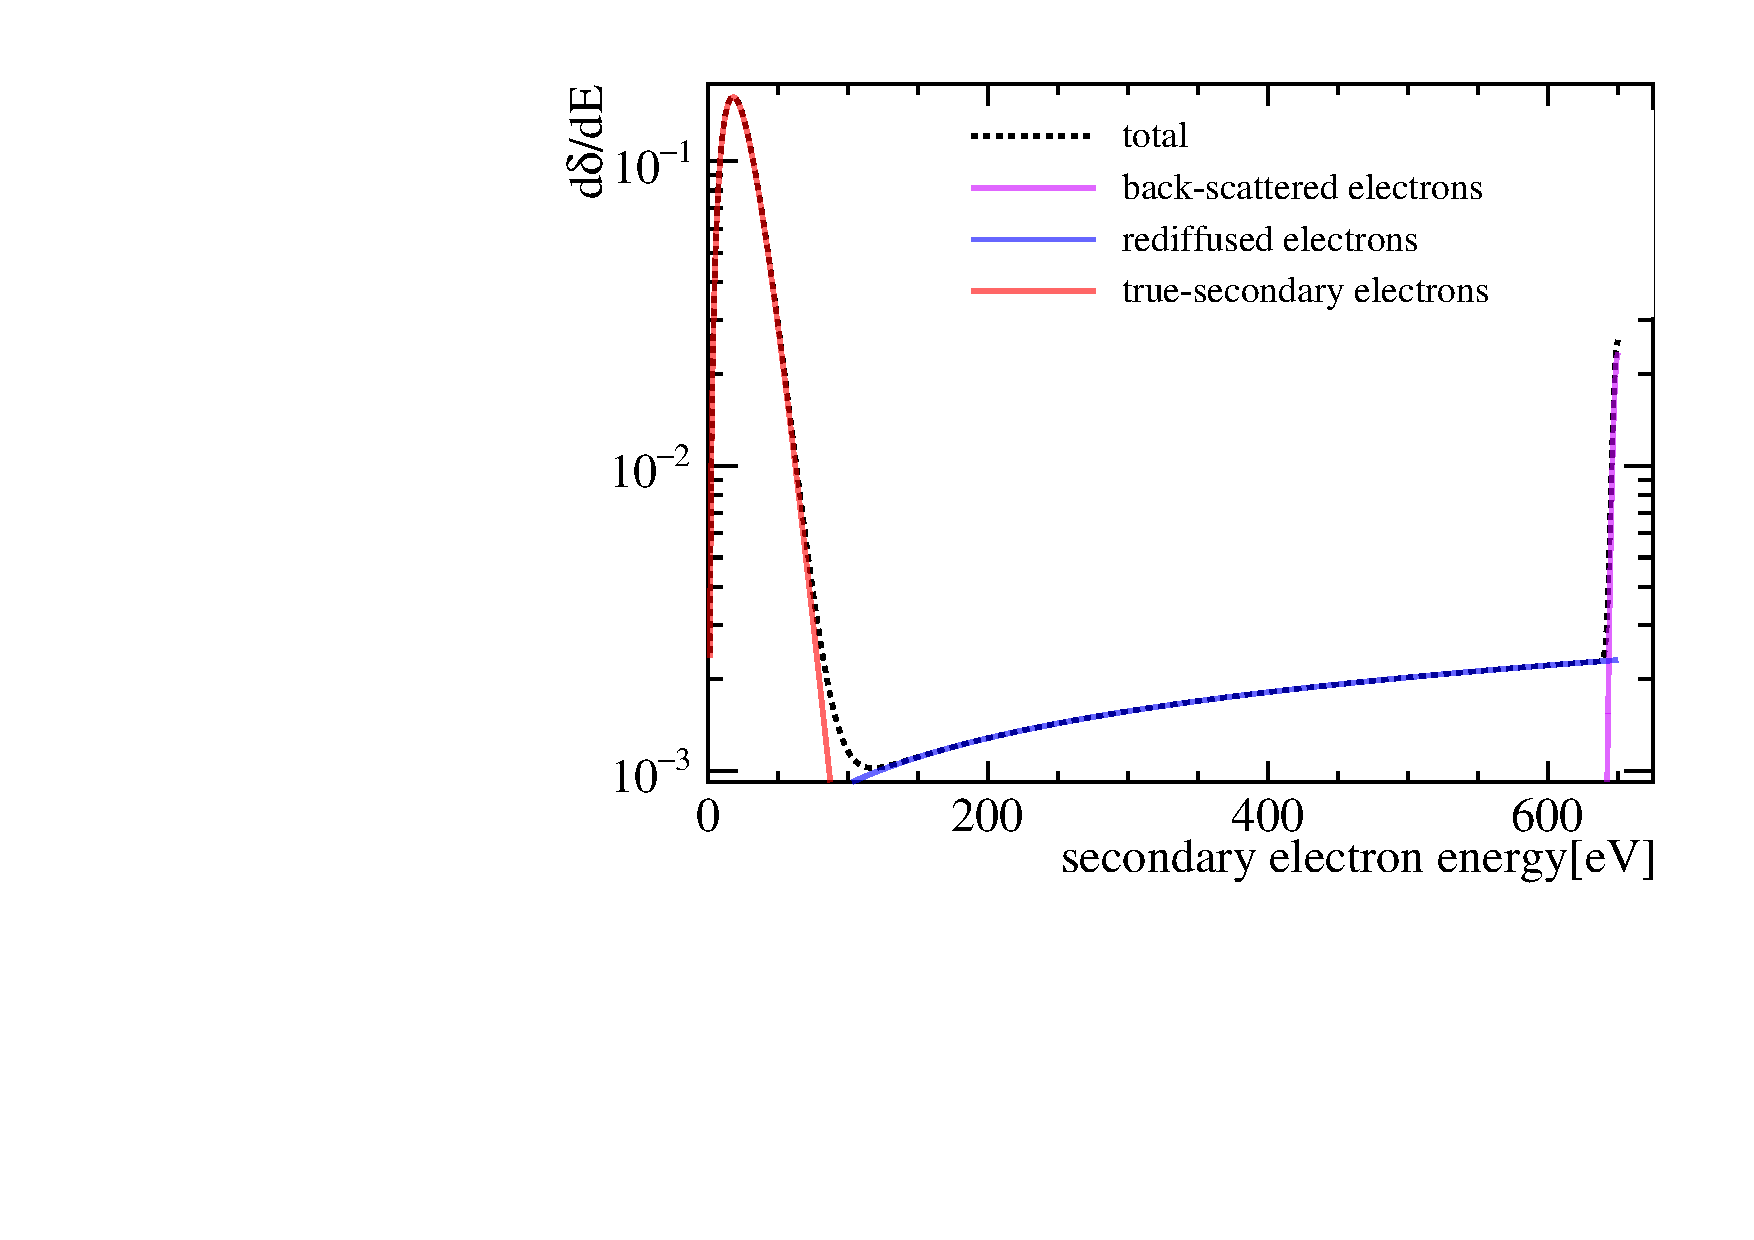
\includegraphics[width=0.5\textwidth]{PMTRelated/GTmodel/SES.pdf}
	\caption{The total energy spectrum of the secondary electrons when the incident energy is \SI{650}{eV}.
		The violet, blue, and red lines represent $\mathrm{d}\delta_{\mathrm{bs}}/\mathrm{d}E$, $\mathrm{d}\delta_{\mathrm{rd}}/\mathrm{d}E$, and
		$\mathrm{d}\delta_{\mathrm{ts}}/\mathrm{d}E$, repectively.
		The black dashed line is $\mathrm{d}\delta/\mathrm{d}E$.}
	\label{fig:SES}
\end{figure}

\subsubsection{An extra multiplication mode}
The MCP-PMT under study uses a Chevron stack of two MCPs as the electron multiplier.
As shown in Fig.~\ref{fig:circuit}, an \ce{Al2O3}-\ce{MgO}-\ce{Al2O3} layer~\cite{zzj2021Al} is deposited
on the channel surface of the lead glass body
and on the entrance electrode M1 of the first MCP through the ALD technology.
There are two alternative routes of amplification for every PE:
the \textit{channel mode}, where the PE directly enters a channel,
and the \textit{surface mode}, where the secondaries from $\mathrm{M}1$ enter the MCP channels under the focusing electric field.
The selection of these two routes is a Bernoulli trial~\cite{1955Scintillation}.

The MCP gain for those low-energy secondaries in the surface mode is substantially
smaller than that for the primary PEs in the channel mode~\cite{2012An}.

\subsubsection{Voltage-division Experiment}\label{sec:gain}
The dependence of the MCP gain for an electron versus its incident energy at the
channel entrance is crucial to understanding the jumbo charges.
We designed a voltage-division experiment to measure such a relationship.

As shown in Fig~\ref{fig:circuit}, we utilized a positive high-voltage power supply~(positive HV) to stabilize the potentials applied
to the MCPs through the circuit~\cite{Luo:2023jdf}.  In parallel, we took a negative high-voltage power supply~(negative HV) to vary the electric
potential difference between the photocathode and $\mathrm{M}1$ to get PEs at different incident energies.
Compared to the experiment of Yang~et~al.~\cite{2017MCP} where the potentials of all the electrodes M1-4
are controllable, our design is a simplified adaptation only to tune the energies of the PEs with commercially available HV products.

\begin{figure}[!ht]
	\centering
	\includegraphics[width=\linewidth]{PMTRelated/GTmodel/set.pdf}
	\caption{
		$\mathrm{M}1$ and $\mathrm{M}3$ are the input electrodes of MCPs, $\mathrm{M}2$ and $\mathrm{M}4$ are the output electrodes,
		and the four electrodes provide the potential differences during operation.
		The PEs directly enter the channels~(channel mode) or hit $\mathrm{M}1$ to produce secondary electrons
		that enter the channels later~(surface mode)~\cite{2016Optimization}. After entering the MCP channel, the electron collides
		with the channel wall many times and is amplified in a series of such multiplications~\cite{1955Scintillation}.
		Our circuit design was modified from the circuit implementation in the reference~\cite{Luo:2023jdf}.
		We removed useless R1 and R2 in our circuit design, while the rest of the resistors remained unchanged.}
	\label{fig:circuit}
\end{figure}

We used a picosecond laser with a wavelength of \SI{405}{nm} to illuminate the MCP-PMT at \SI{1}{kHz} rate and feed an electronic trigger signal to capture waveform data.
To obtain the single PE, we adjusted the intensity of the laser until the occupancy was below 0.1.
We deployed a 10-bit oscilloscope~(HDO9000 with HD1024 Technology)~\cite{teledynelecroy} to capture the \SI{100}{ns} waveform
with a sampling rate of \SI{40}{GS/s} and a range of [-20, 60]~\si{mV}.

We obtained the gain of the MCP-PMTs at different energies of the incident electrons by fitting the Gaussian on the charge distribution,
and conducted the same experiment on two MCP-PMTs with~(Fig.~\ref{fig:gain_ald}) and without~(Fig.~\ref{fig:gain_noald})
\ce{Al2O3}-\ce{MgO} deposited on $\mathrm{M}1$ to contrast the effect of the surface mode.
The positive voltages for the MCP-PMT with and without \ce{Al2O3}-\ce{MgO} on M1 are +\SI{1205}{V} and  +\SI{1240}{V}, respectively.
The initial energies of the PEs are \SI{\sim 1}{eV}~\cite{Nathan1970TheED}
and the systematic error of the negative HV itself is within \SI{2}{V}.
The incident energies~($E_0$) are defined as the energies acquired by the PEs in the electric field,
numerically equal to the potential difference between the photocathode and M1, with an error of $\pm$\SI{2}{eV}.
We scanned the MCP gain and measured it every \SI{10}{eV} when $10\leqslant E_0<100$~\si{eV}, every \SI{20}{eV} when $100\leqslant E_0<200$~\si{eV}
and every \SI{50}{eV} when $200<E_0\leqslant 650$~\si{eV}.
For the MCP-PMT with \ce{Al2O3}-\ce{MgO} deposited on M1, our scan range is $10\leqslant E_0\leqslant 600$~\si{eV}.
For the MCP-PMT without, the range is $10\leqslant E_0\leqslant 680$~\si{eV}.

The charges of the captured waveforms were measured with \emph{fast stochastic matching pursuit}~(FSMP)~\cite{Xu_2022,Wang_2024},
which suppresses the interference of electronic noise to give accurate charge spectra under a wide range of gain.
Due to FSMP's ability to count PEs, the charge would be 0 when $n_{\mathrm{PE}}=0$
and the pedestal is cleanly cut out in the output charge distribution.
In Fig.~\ref{fig:gain_fit}, the peaks are attributed to the channel mode.
The jumbo charges from the surface mode are to the right and deficient amplifications
are to the left of the peaks.
Due to the small contribution of secondaries from the surface mode for the MCP-PMT without \ce{Al2O3}-\ce{MgO} deposited on $\mathrm{M}1$,
there is no jumbo charge in the charge spectrum, as shown in Fig.~\ref{fig:gain_noald}.
To obtain the MCP gain for the electrons directly entering the channels,
we only fitted the peak to exclude the influence of the surface mode.

We obtained approximate values of $\mu_{\mathrm{p}}$ and $\sigma_{\mathrm{p}}$ of the charge distribution to
provide initial values and ranges for a detailed fit.
The fit ranges were determined from the incident energies of the PEs,
when $E_0>100$~\si{eV}, it was $[\mu_{\mathrm{p}}-1.3\sigma_{\mathrm{p}}, \mu_{\mathrm{p}}+1.6\sigma_{\mathrm{p}}]$;
when $30<E_0\leqslant 100$~\si{eV}, $[\mu_{\mathrm{p}}-0.8\sigma_{\mathrm{p}}, \mu_{\mathrm{p}}+1.6\sigma_{\mathrm{p}}]$;
and when $E_0\leqslant 30$~\si{eV}, $[\mu_{\mathrm{p}}-1.5\sigma_{\mathrm{p}}, \mu_{\mathrm{p}}+1.8\sigma_{\mathrm{p}}]$.
It is sufficient to extract the mean charge $\mu(E_0)$ and the standard deviation $\sigma(E_0)$
of the channel-mode peak to measure the MCP gain for electrons at different energies.

\begin{figure}[!ht]
	\centering
	\begin{subfigure}[b]{0.48\textwidth}
		\centering
		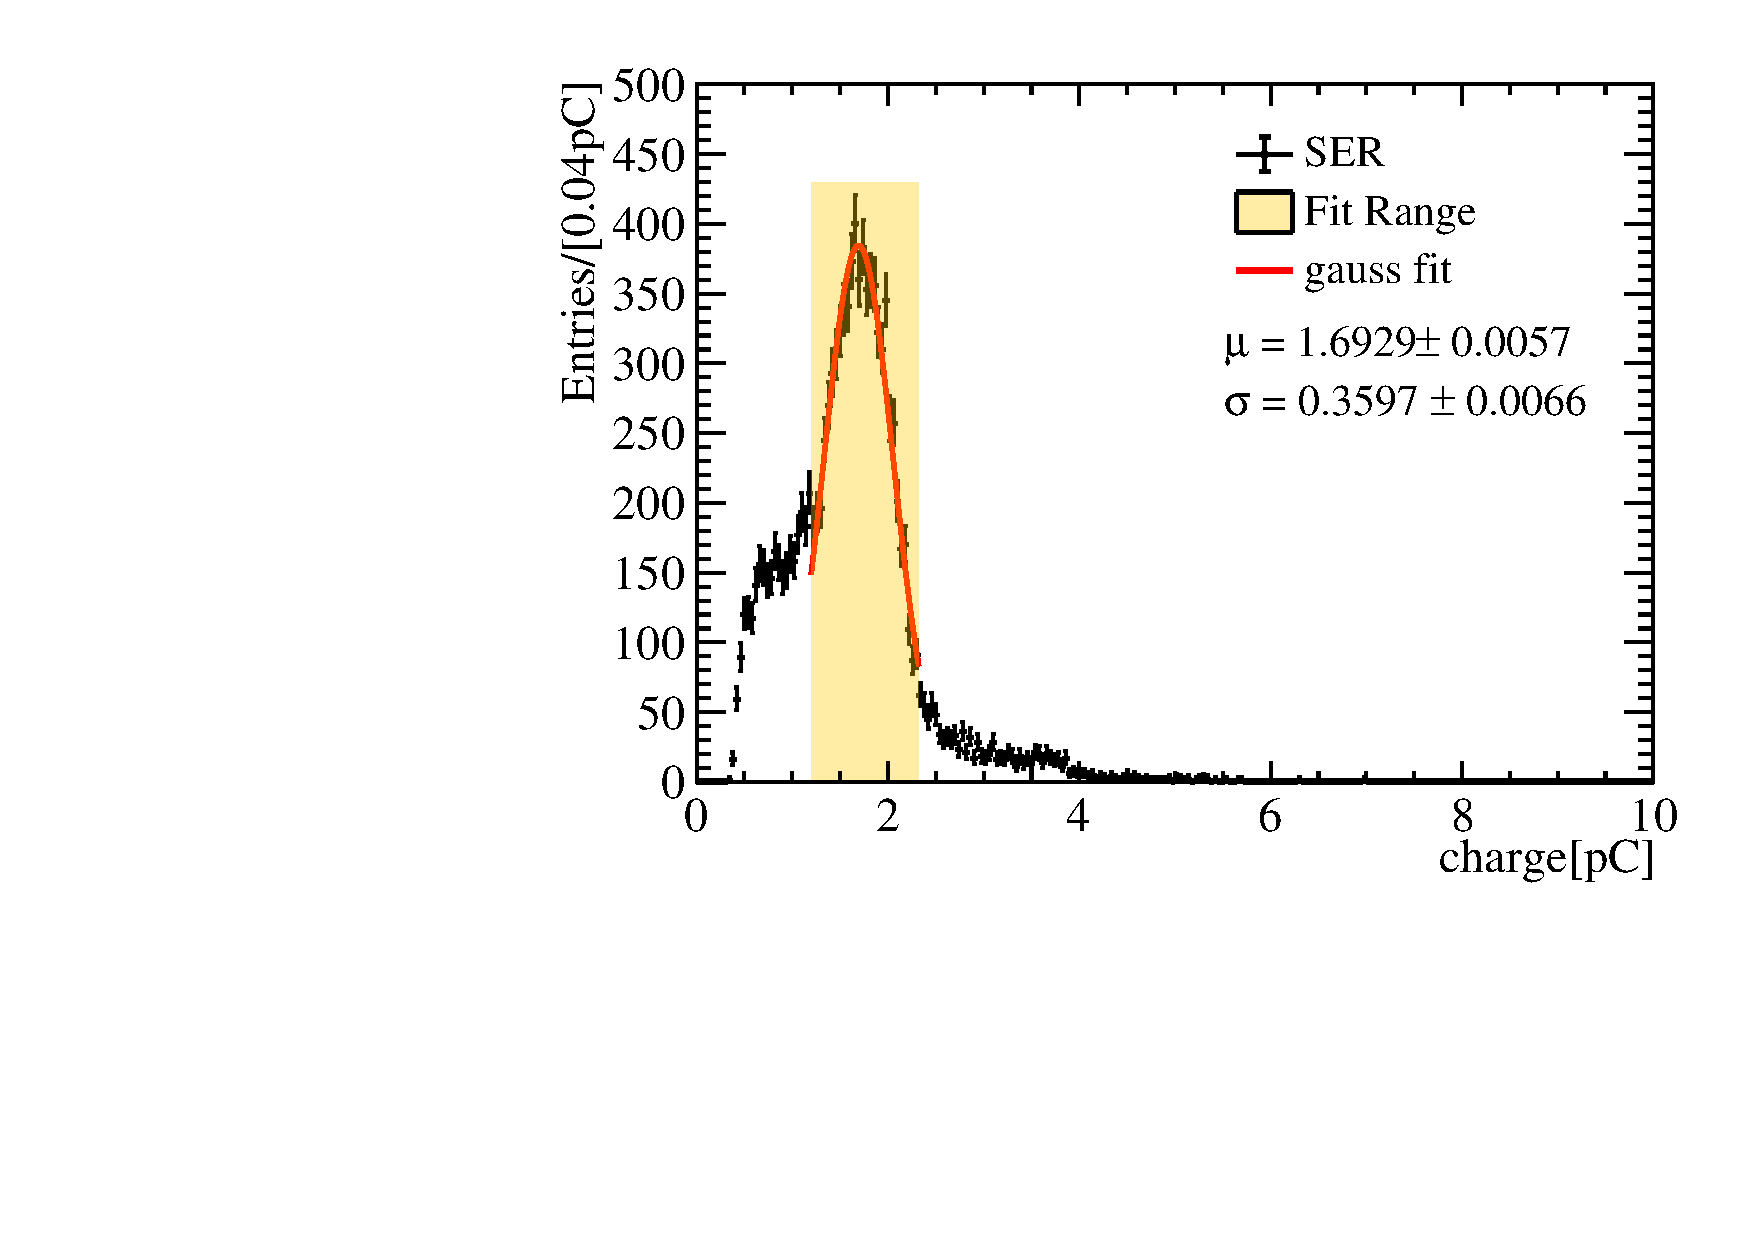
\includegraphics[width=\textwidth]{PMTRelated/GTmodel/fit_noald.pdf}
		\caption{}
		\label{fig:gain_noald}
	\end{subfigure}
	\hfill
	\begin{subfigure}[b]{0.48\textwidth}
		\centering
		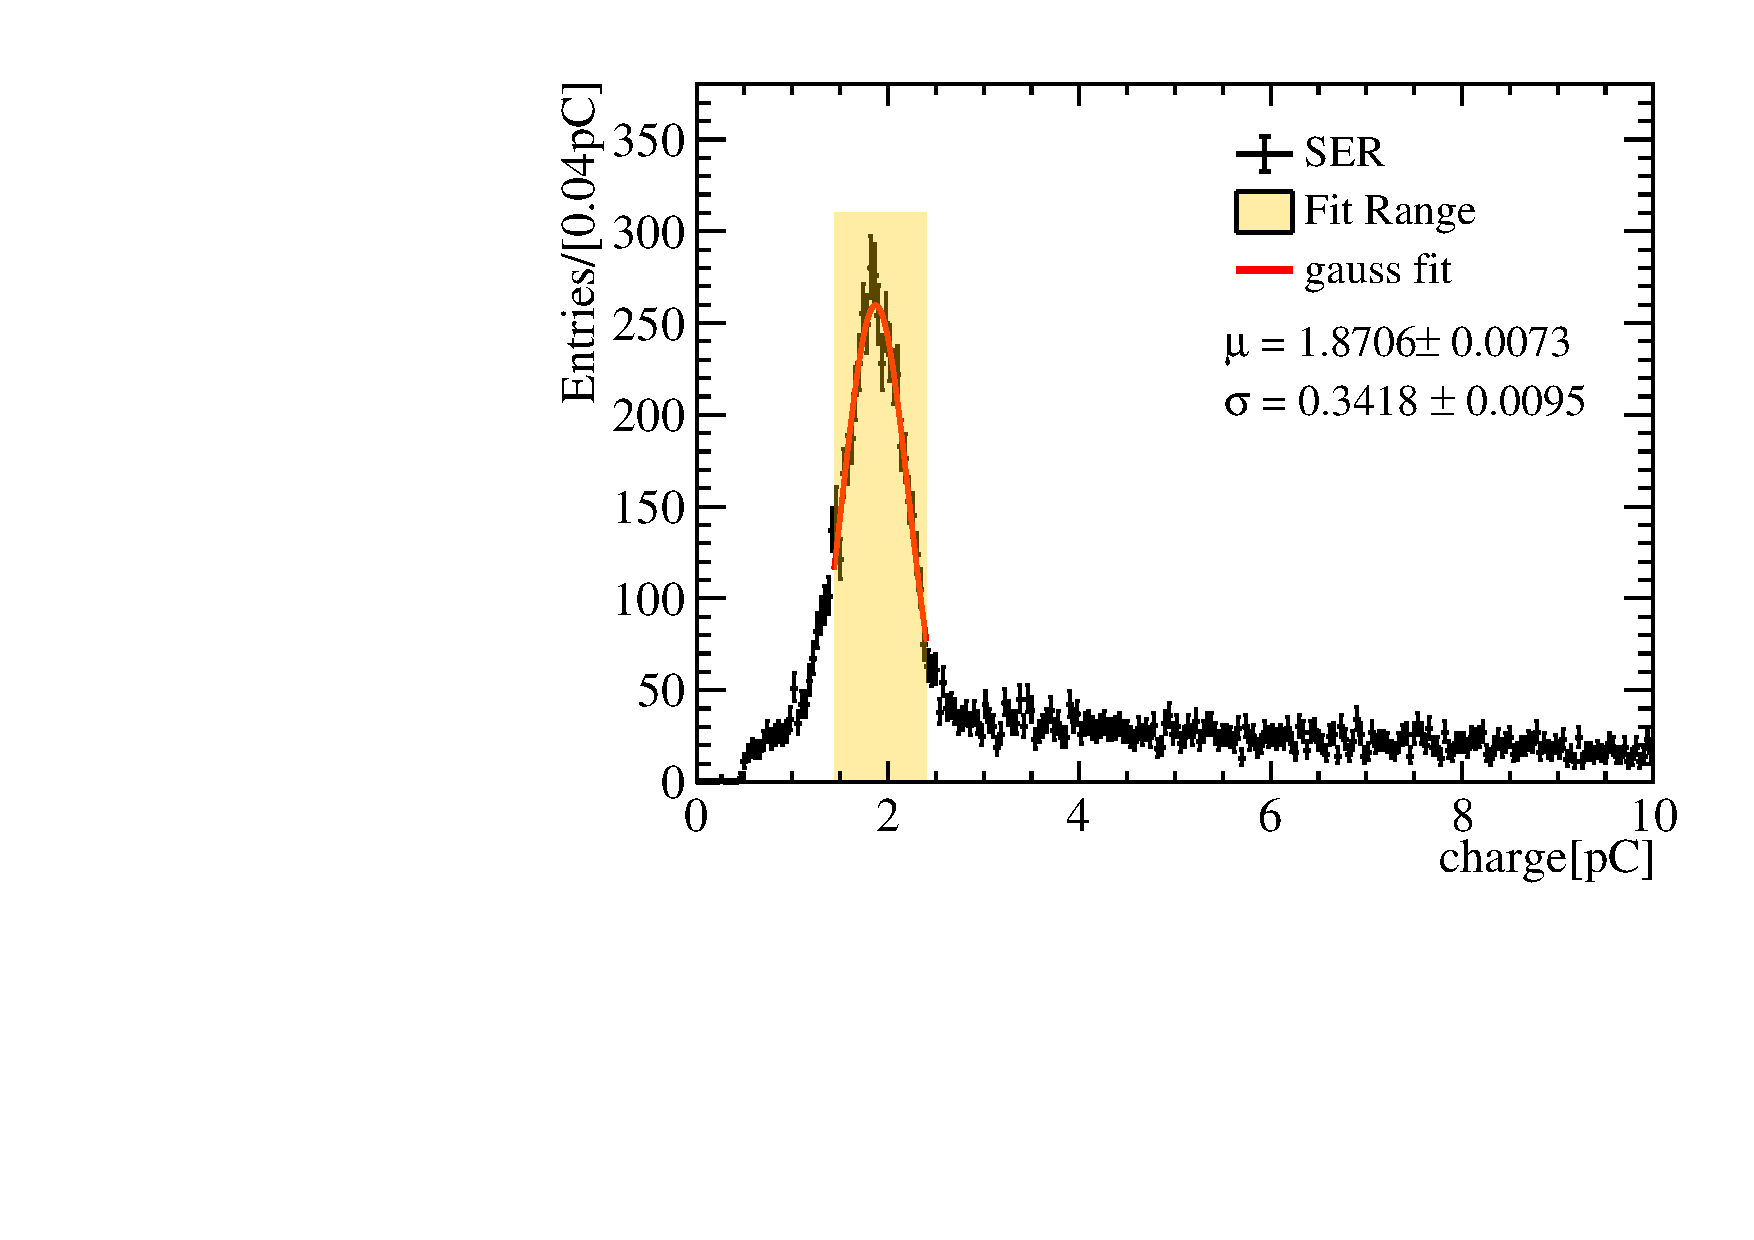
\includegraphics[width=\textwidth]{PMTRelated/GTmodel/fit_ald.pdf}
		\caption{}
		\label{fig:gain_ald}
	\end{subfigure}

	\caption{Fit of the charge spectrum of the MCP-PMT without \subref{fig:gain_noald} and with \subref{fig:gain_ald}
		\ce{Al2O3}-\ce{MgO} deposited on $\mathrm{M}1$.
		We observed that \subref{fig:gain_noald} does not exhibit jumbo charges.
		The yellow areas are incident energy-dependent intervals and
		the red lines are fitting results of the Gaussian functions in the intervals.
	}
	\label{fig:gain_fit}
\end{figure}

After fitting with Gaussians, we interpolate and extrapolate linearly to obtain the relations of $\mu(E_0)$ and $\sigma(E_0)$ in Fig.~\ref{fig:gaintest}.
The difference in the relations of MCP-PMTs with and without \ce{Al2O3}-\ce{MgO} deposited on $\mathrm{M}1$ comes from the influence of the charge contributed from the surface mode.
When \(E_0 < \SI{200}{eV}\), \(\mu(E_0)\) rapidly increases.
As \(E_0 > \SI{200}{eV}\), \(\mu(E_0)\) gradually stabilizes.
The $\sigma(E_0)$ is overall increasing similar to $\mu(E_0)$ but sees a drop around \SI{200}{eV}.
A similar trend of \(\mu(E_0)\) is reported by Yang~et~al.~\cite{2017MCP}.
In our case, the best relative resolution \(\sigma/\mu\) is at around \SI{600}{eV} and
Yang~et~al.'s results suggested \SI{200}{eV}.
Cao~et~al.\cite{cao_secondary_2021} found that the SEY of \ce{Al2O3}-\ce{MgO}
increases with the incident energy in 100--\SI{600}{eV}.
Even though the film structure and thickness we used are different,
we can still make a rough assessment that
the trend of $\sigma/\mu$ obtained here is reasonable,
considering the variation curves of the SEY of \ce{Al2O3} and \ce{MgO} with energy.
\begin{figure}[!ht]
	\centering
	\begin{subfigure}[b]{0.45\textwidth}
		\centering
		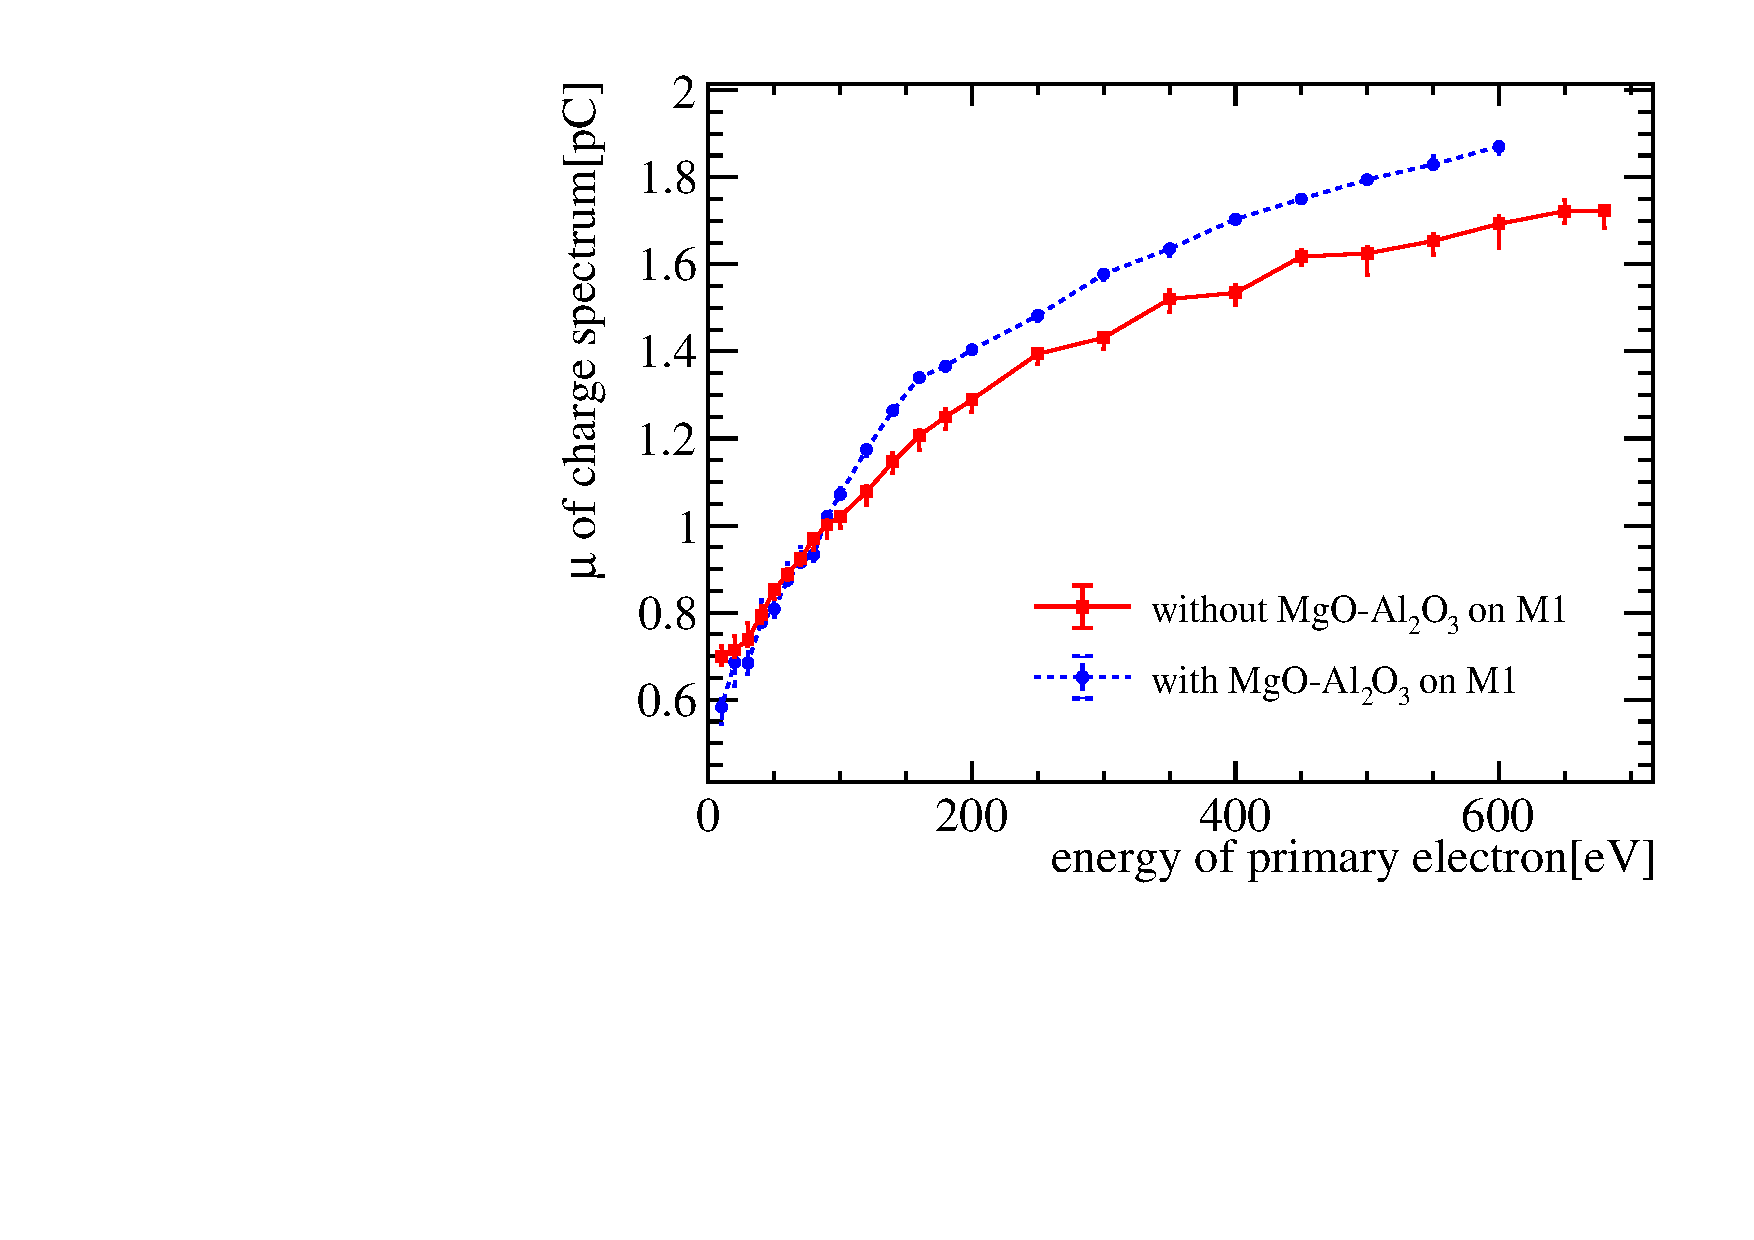
\includegraphics[width=\textwidth]{PMTRelated/GTmodel/gain_mu.pdf}
		\caption{}
		\label{fig:gain}
	\end{subfigure}%
	\begin{subfigure}[b]{0.45\textwidth}
		\centering
		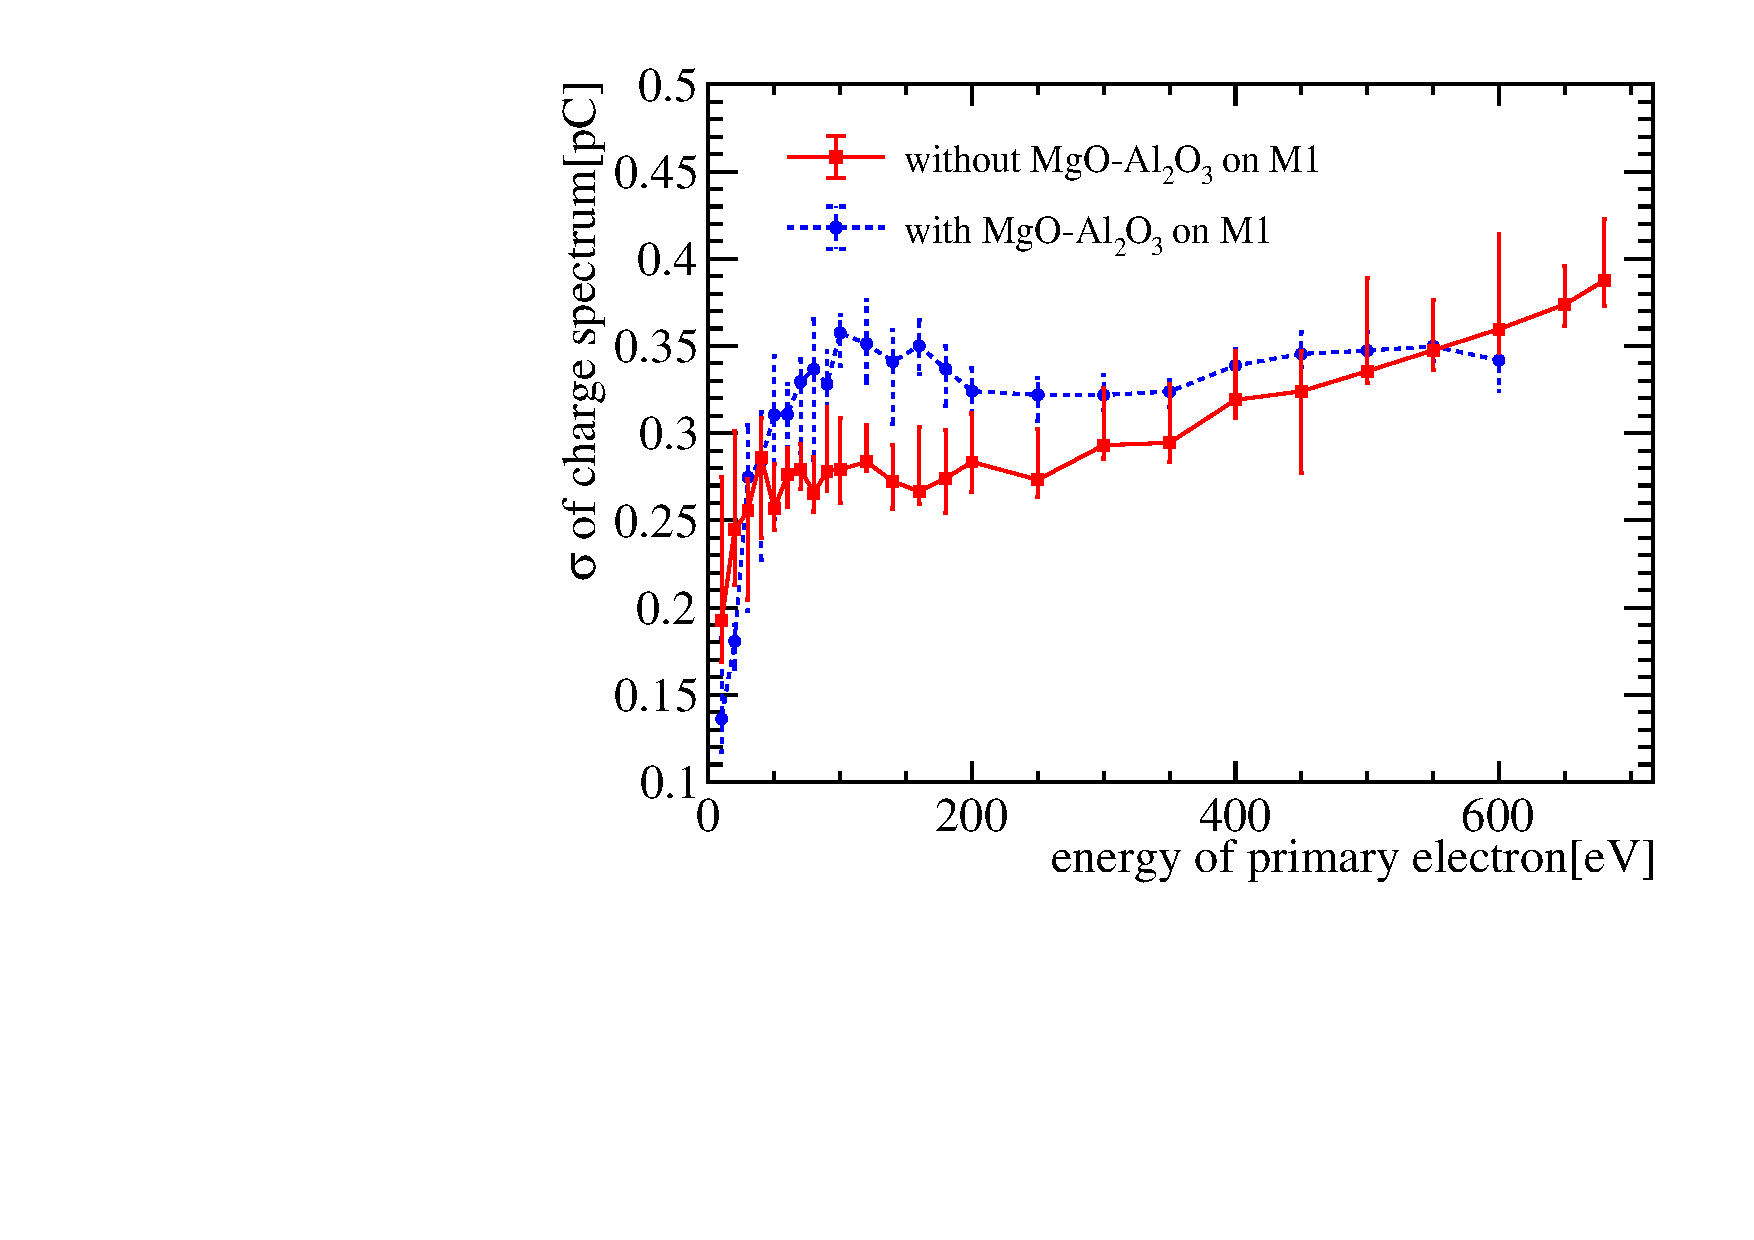
\includegraphics[width=\textwidth]{PMTRelated/GTmodel/gain_sigma.pdf}
		\caption{}
		\label{fig:sigma}
	\end{subfigure}
	\hfill
	\begin{subfigure}[b]{0.45\textwidth}
		\centering
		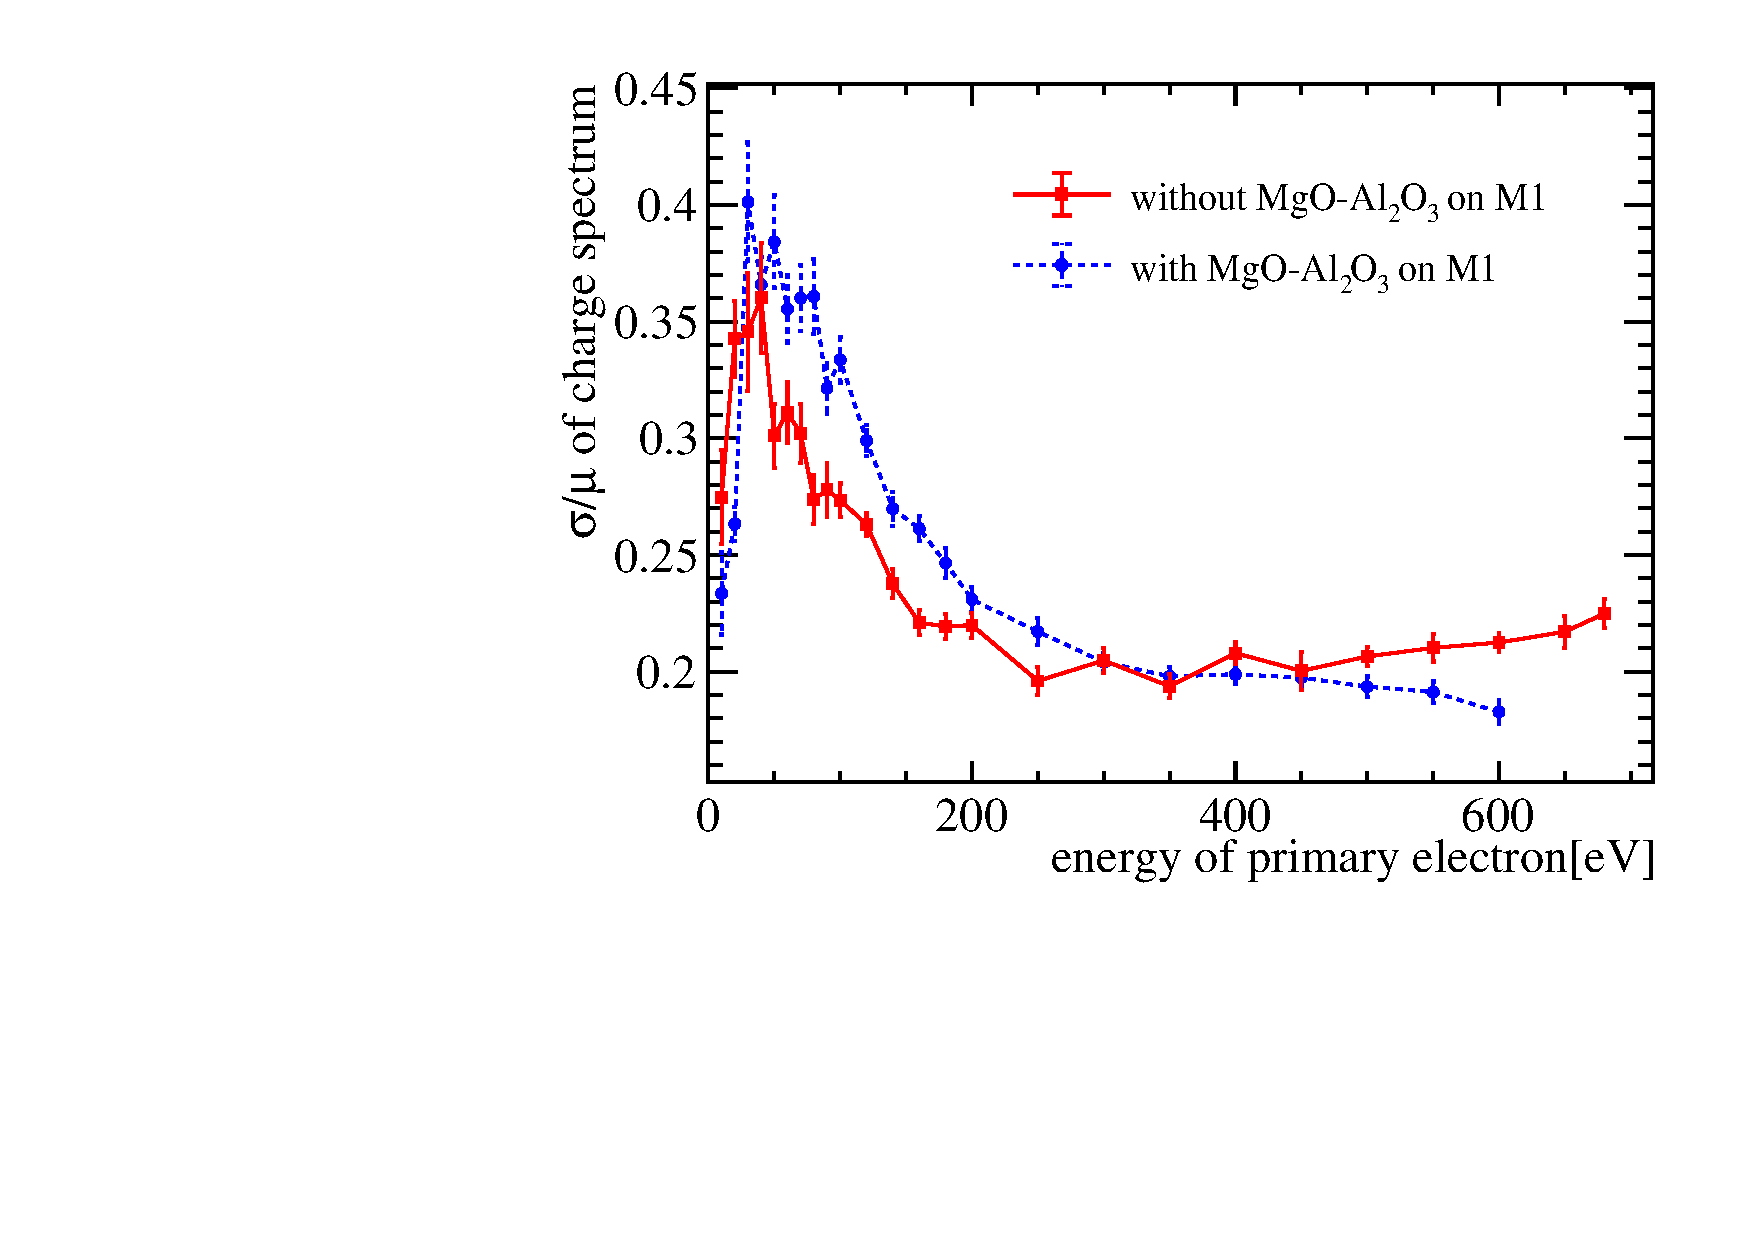
\includegraphics[width=\textwidth]{PMTRelated/GTmodel/gain_sigmamu.pdf}
		\caption{}
		\label{fig:sigmamu}
	\end{subfigure}
	\caption{\subref{fig:gain} The mean \(\mu\) increases as the incoming electron energy~$E_0$ increases.
		\subref{fig:sigma} The standard deviation \(\sigma\) changes with energy.
		The MCP-PMT with \ce{Al2O3}-\ce{MgO} deposited on $\mathrm{M}1$~(the red line) shows a similar variation trend to the one without~(the blue line).
		\subref{fig:sigmamu} The resolution $\sigma/\mu$ increases between 0-\SI{50}{eV}, decreases between 50-\SI{400}{eV},
		and after \SI{400}{eV}, there is a slight decrease for those with \ce{Al2O3}-\ce{MgO} deposited on $\mathrm{M}1$ ~(the blue line) and a slight increase for those without~(the red line).
	}
	\label{fig:gaintest}
\end{figure}

\subsubsection{Charge-Spectra Decomposition}\label{sec:convolution}
The Furman model in Sec.~\ref{subsec:fuman} predicts the energies of the secondaries.
Our voltage-division experiment in Sec.~\ref{sec:gain} measured the relationship between the
MCP gain and the incident energies of the electrons.
We follow the flowchart in Fig.~\ref{fig:process} to calculate the charge distribution by Monte Carlo.
In this study, we shone the laser at the apex of the photocathode hemisphere,
and the PEs hit M1 with an incident angle~$\theta_0=0^\circ$.
The complex amplification process in the channels is described by
the incident energy-dependent Gamma distributions $\varGamma(\alpha(E), \beta(E))$ described in Sec.~\ref{gammapossion}. The $\alpha(E)$ and $\beta(E)$ are estimated with the relations of $\mu(E)$ and $\sigma(E)$ of MCP-PMT without \ce{Al2O3}-\ce{MgO} coating on the input electrode, which eliminates the influence of the surface mode.
\begin{figure}[!ht]
	\centering
	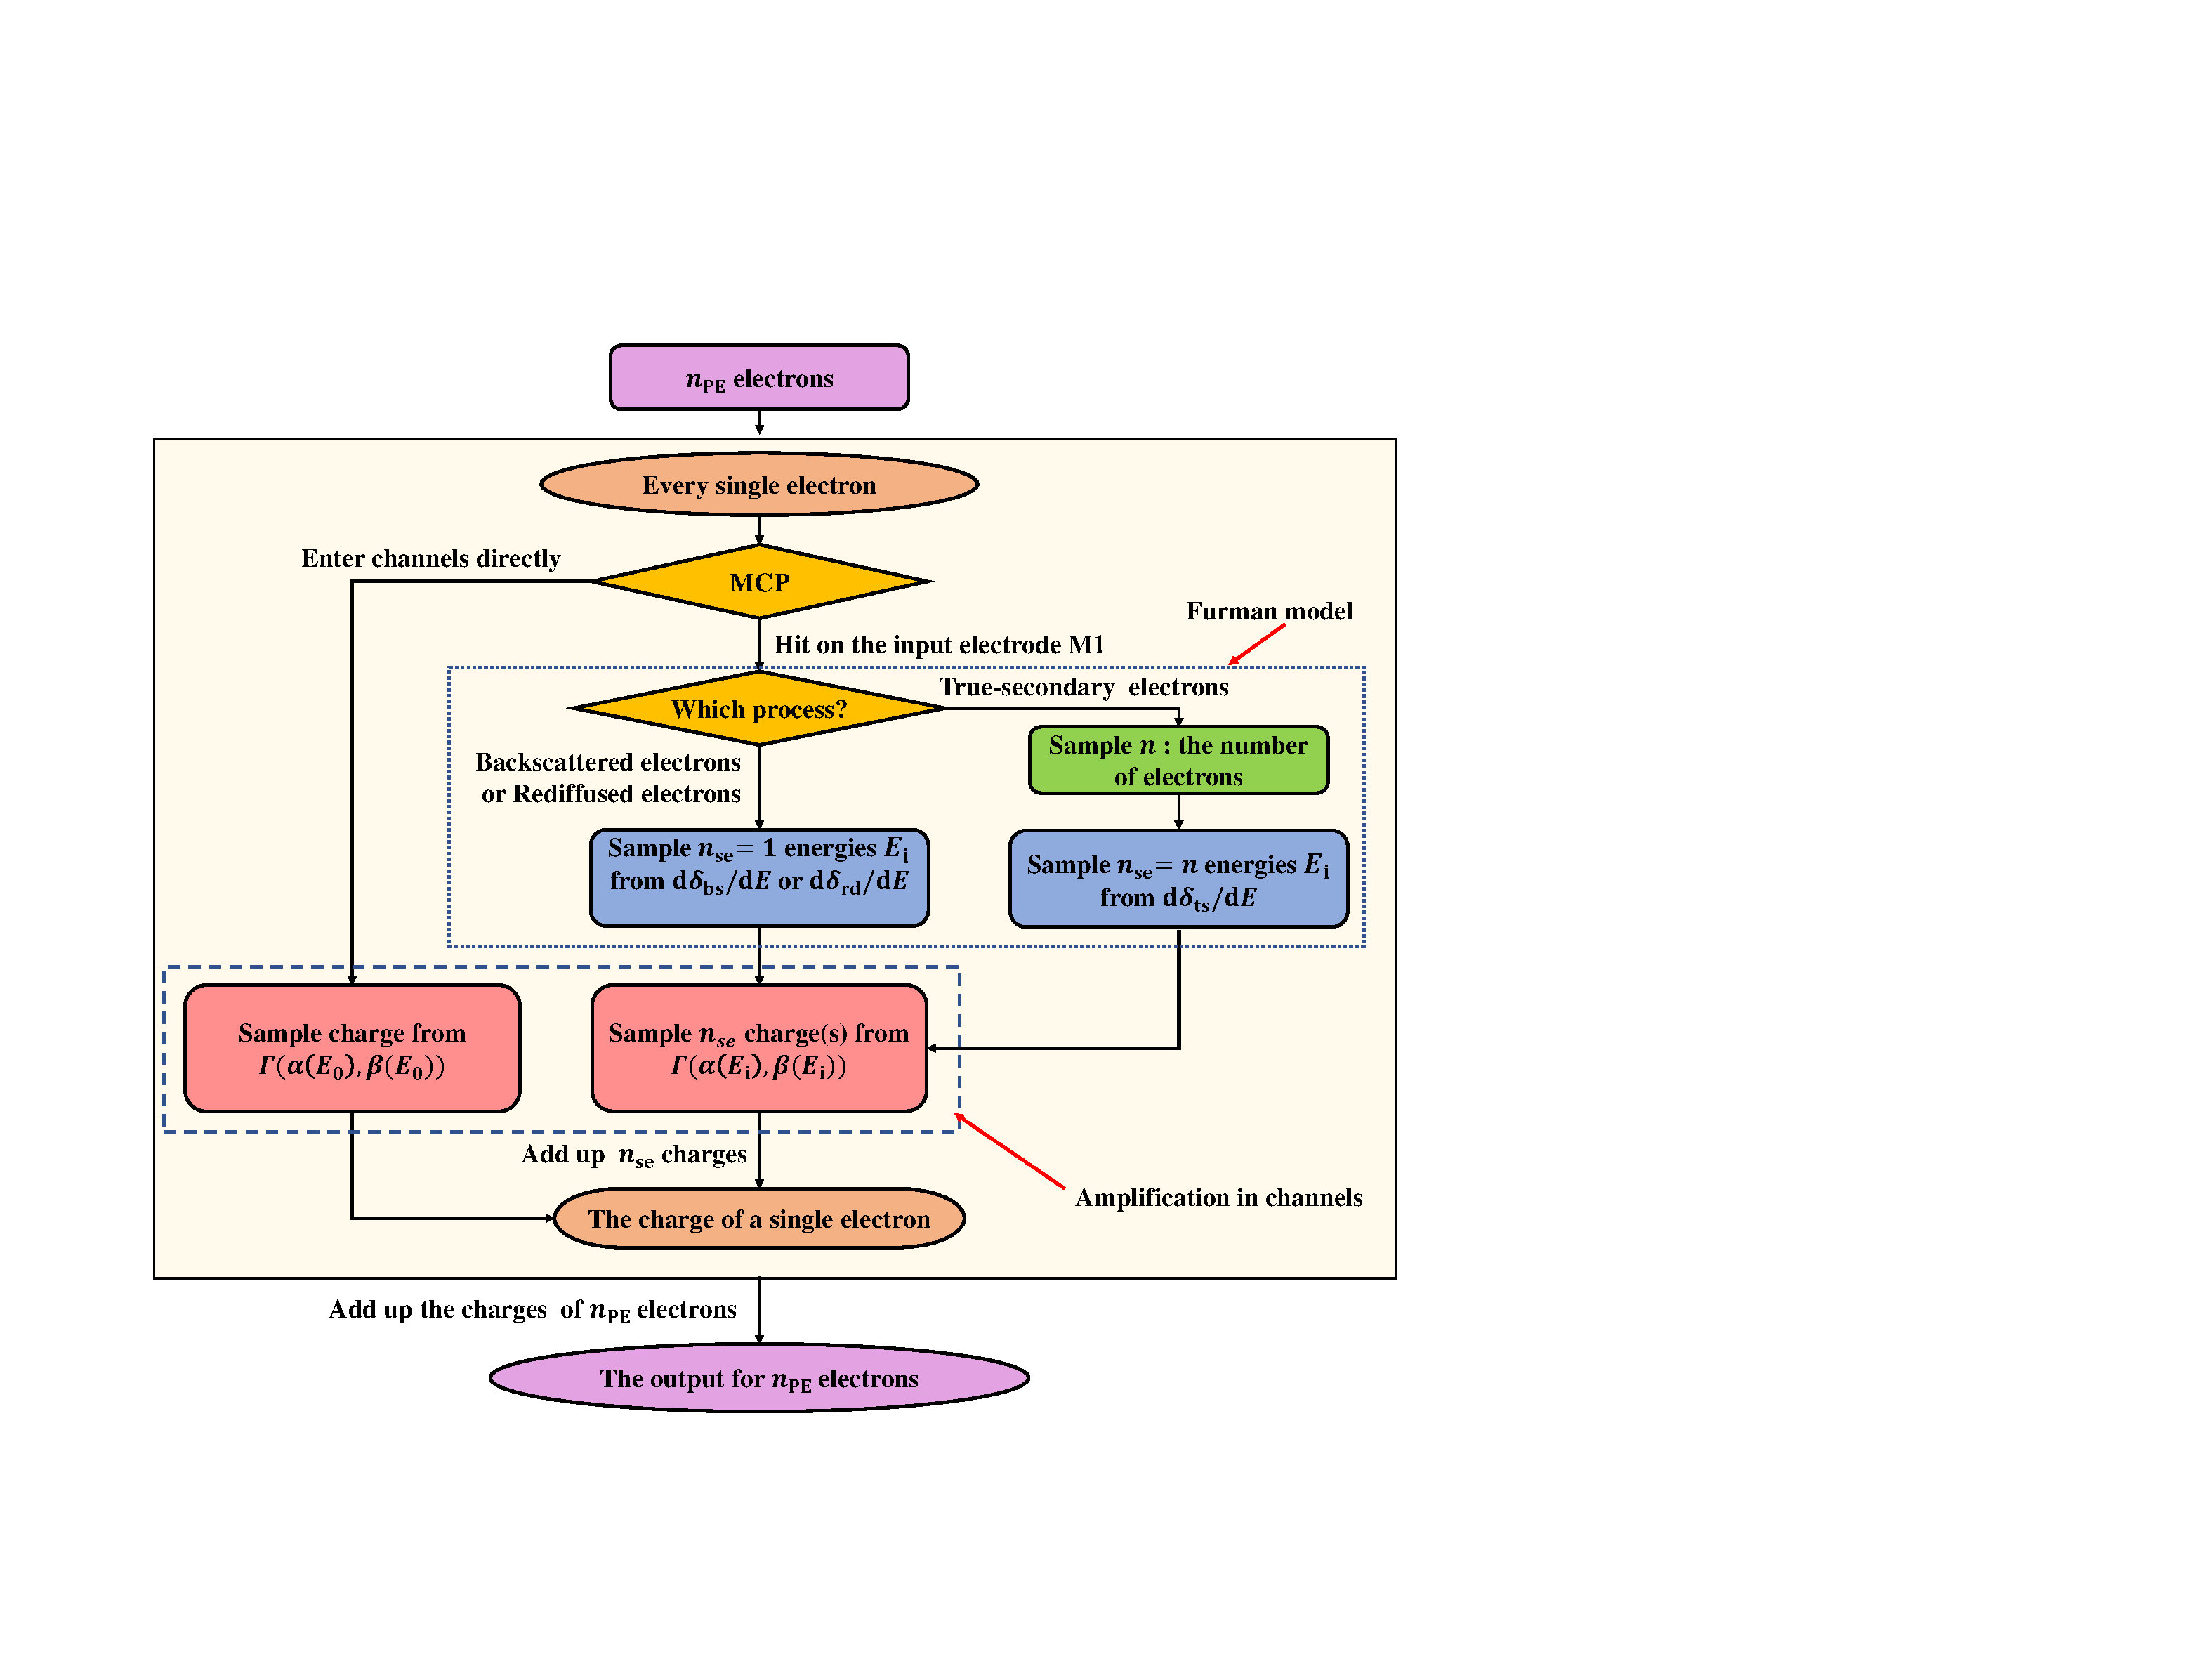
\includegraphics[width=\linewidth]{PMTRelated/GTmodel/process.pdf}
	\caption{The flowchart of Monte Carlo to compute the charge spectrum.
		The output charge consists of $n_\mathrm{PE}$ SER charges.
		The PEs in the channel mode enter channels directly, while PEs in the surface mode hit the input electrode.
		The energies of the $n_\mathrm{se}$ secondaries in the surface mode are sampled from the Furman model.
		The amplification in channels is modeled by the incident energy-dependent Gamma distribution.
	}
	\label{fig:process}
\end{figure}
Taking into account the light intensity, we repeatedly sample $n_{\mathrm{PE}}$ from the Poisson distribution
and sum up $n_{\mathrm{PE}}$ SER charges for the output to get a spectrum.

For sampling an SER charge, we assign the probabilities of the channel and surface
modes as $p$ and $1-p$ for a Bernoulli trial. The SER charge spectrum $f_{\text{MCP-PMT}}(Q)$ is
\begin{equation}
	\label{eq:convolution}
	f_{\text{MCP-PMT}}(Q) = p f_{\mathrm{ch}}(Q)+(1-p) f_{\mathrm{surf}}(Q)
\end{equation}
where $f_{\mathrm{ch}}(Q)$ and $f_{\mathrm{surf}}(Q)$ are the charge distributions of the channel and surface modes.
$f_{\mathrm{ch}}(Q)$ is set to \(f_\Gamma(Q; \alpha(E_0), \beta(E_0))\), with the incident energy being \SI{650}{eV}.
The factors \(\alpha(E_0), \beta(E_0)\) are converted from $\mu(E_0)$ and $\sigma(E_0)$ without \ce{Al2O3}-\ce{MgO} coating in Fig.~\ref{fig:gaintest}.

The \(f_{\mathrm{surf}}(Q)\) is divided into three components by the Furman model
corresponding to Eqs.~(\ref{eq:backscatter})--(\ref{eq:true}),
$f_{\mathrm{bs}}(Q)$ for the back-scattered electrons,
$f_{\mathrm{rd}}(Q)$ for the rediffused electrons,
and $f_{\mathrm{ts}}(Q)$ for the true-secondary electrons.
\begin{equation}
	\label{eq:surface_3}
	\begin{aligned}
		f_{\mathrm{surf}}(Q) & = p_{\mathrm{bs}} f_{\mathrm{bs}}(Q) + p_{\mathrm{rd}} f_{\mathrm{rd}}(Q) + (1- p_{\mathrm{bs}} - p_{\mathrm{rd}}) f_{\mathrm{ts}}(Q)                     \\
		                     & = \delta_{\mathrm{bs}} f_{\mathrm{bs}}(Q) + \delta_{\mathrm{rd}} f_{\mathrm{rd}}(Q) + (1- \delta_{\mathrm{bs}} - \delta_{\mathrm{rd}}) f_{\mathrm{ts}}(Q) \\
	\end{aligned}
\end{equation}
where $p_{\mathrm{bs}}$ and $p_{\mathrm{rd}}$ are the mixture ratios
determined by the composition and thickness of surface emissive material
that varies among the PMTs.  Furman and Pivi~\cite{2002Probabilistic} assume that
only one electron is emitted in back-scattered mode and rediffused mode
so that \(\delta_{\mathrm{bs}} = p_{\mathrm{bs}}\) and \(\delta_{\mathrm{rd}} = p_{\mathrm{rd}}\).
In the calculation, we specify $\delta_{\mathrm{rd}}=0.09$ and $\delta_{\mathrm{bs}}=0.01$.
The energy of the back-scattered electron is nearly equal to that of the PEs in the channel mode,
and so is the MCP gain for them.
The energy of the rediffused electron
is lower -- from \SIrange{100}{600}{eV}, causing the charge after MCP multiplication
to be slightly smaller thanks to the relatively slow increase of gain in that range in Fig.~\ref{fig:gain}.
Either contributes a single electron and is practically indistinguishable from
the channel mode in the charge spectra. Such a degeneracy is summarized in Eq.~\eqref{eq:gammaTweedie}:
\begin{equation}
	\label{eq:gammaTweedie}
	\begin{aligned}
		f_{\text{MCP-PMT}}(Q) & = p f_{\mathrm{ch}}(Q) + (1-p) f_{\mathrm{surf}}(Q)                                                                                                                                    \\
		                      & = p f_{\mathrm{ch}}(Q)+(1-p) [\delta_{\mathrm{bs}} f_{\mathrm{bs}}(Q) + \delta_{\mathrm{rd}} f_{\mathrm{rd}}(Q) + (1- \delta_{\mathrm{bs}} - \delta_{\mathrm{rd}}) f_{\mathrm{ts}}(Q)] \\
		                      & = [p + (1-p)(\delta_{\mathrm{bs}} + \delta_{\mathrm{rd}})] f_{\mathrm{ch}}(Q) + (1-p)(1-\delta_{\mathrm{bs}} - \delta_{\mathrm{rd}})f_{\mathrm{ts}}(Q)
	\end{aligned}
\end{equation}
where the spectra $f_{\mathrm{ch}}(Q)$, $f_{\mathrm{rd}}(Q)$ and $f_{\mathrm{bs}}(Q)$ are
merged into $f_{\mathrm{ch}}(Q)$.

Nevertheless, Eq.~(\ref{eq:gammaTweedie}) is incomplete.
We should consider the case when the secondaries hit the MCP surface again.
The round trip does not inject extra energy.
A back-scattered or rediffused secondary gets amplified essentially in the same way
as a primary PE, while a true-secondary electron has too low energy to multiply again.
Therefore, \(p_0\), the net contribution to \(f_{\mathrm{ch}}(Q)\), is a geometric series
\begin{equation}
	\label{eq:p0}
	p_0 = p \sum_{{i}=0}^\infty [(1-p) (\delta_{\mathrm{bs}} + \delta_{\mathrm{rd}})]^{i} = \frac{p}{1 - (1-p) (\delta_{\mathrm{bs}} + \delta_{\mathrm{rd}})}
\end{equation}
and \(f_{\mathrm{ts}}(Q)\) gets \(\frac{(1-p)(1-\delta_{\mathrm{bs}} - \delta_{\mathrm{rd}})}{1 - (1-p) (\delta_{\mathrm{bs}} + \delta_{\mathrm{rd}})}\) or \(1-p_0\).
Eq.~(\ref{eq:gammaTweedie}) is remarkably reduced to
\begin{equation}
	\label{eq:1}
	f_{\text{MCP-PMT}}(Q) = p_0 f_{\mathrm{ch}}(Q) + (1-p_0) f_{\mathrm{ts}}(Q).
\end{equation}

In the case of the true-secondary electrons, their count $n$ follows a Poissonian. The sum of the sampled $n$ charges
serves as the output \(Q_{\mathrm{ts}}\),
\begin{equation}
	\label{eq:ts_all}
	\begin{aligned}
		 & Q_{\mathrm{ts}} = \sum_{i=1}^{n} Q_{i}            \\
		 & n \sim \mathrm{\pi}(\delta_{\mathrm{ts}}')        \\
		 & Q_{i} \sim \varGamma[\alpha(E_{i}), \beta(E_{i})] \\
	\end{aligned}
\end{equation}
where \(E_{i}\) are sampled from Eq.~(\ref{eq:true}).
$\alpha(E_{i})$ and $\beta(E_{i})$ are converted from
\(\mu(E_{i})\) and \(\sigma(E_{i})\) of Fig.~\ref{fig:gaintest}.
For completeness, \(\delta_\mathrm{ts} = (1-\delta_{\mathrm{bs}} - \delta_{\mathrm{rd}})\delta_{\mathrm{ts}}'\)
is the electric-current ratio of the true-secondary electrons to that of the primary.

The charge spectra of different $n$ are shown in Fig.~\ref{fig:true_n}.
Due to the lower energies of the secondaries, their charges are smaller.
It is challenging to distinguish each charge formed at the anode,
as multiple secondary electrons enter the MCP channels simultaneously.
Bigger $n$ results in a larger charge.

\begin{figure}[!htbp]
	\begin{subfigure}{0.47\linewidth}
		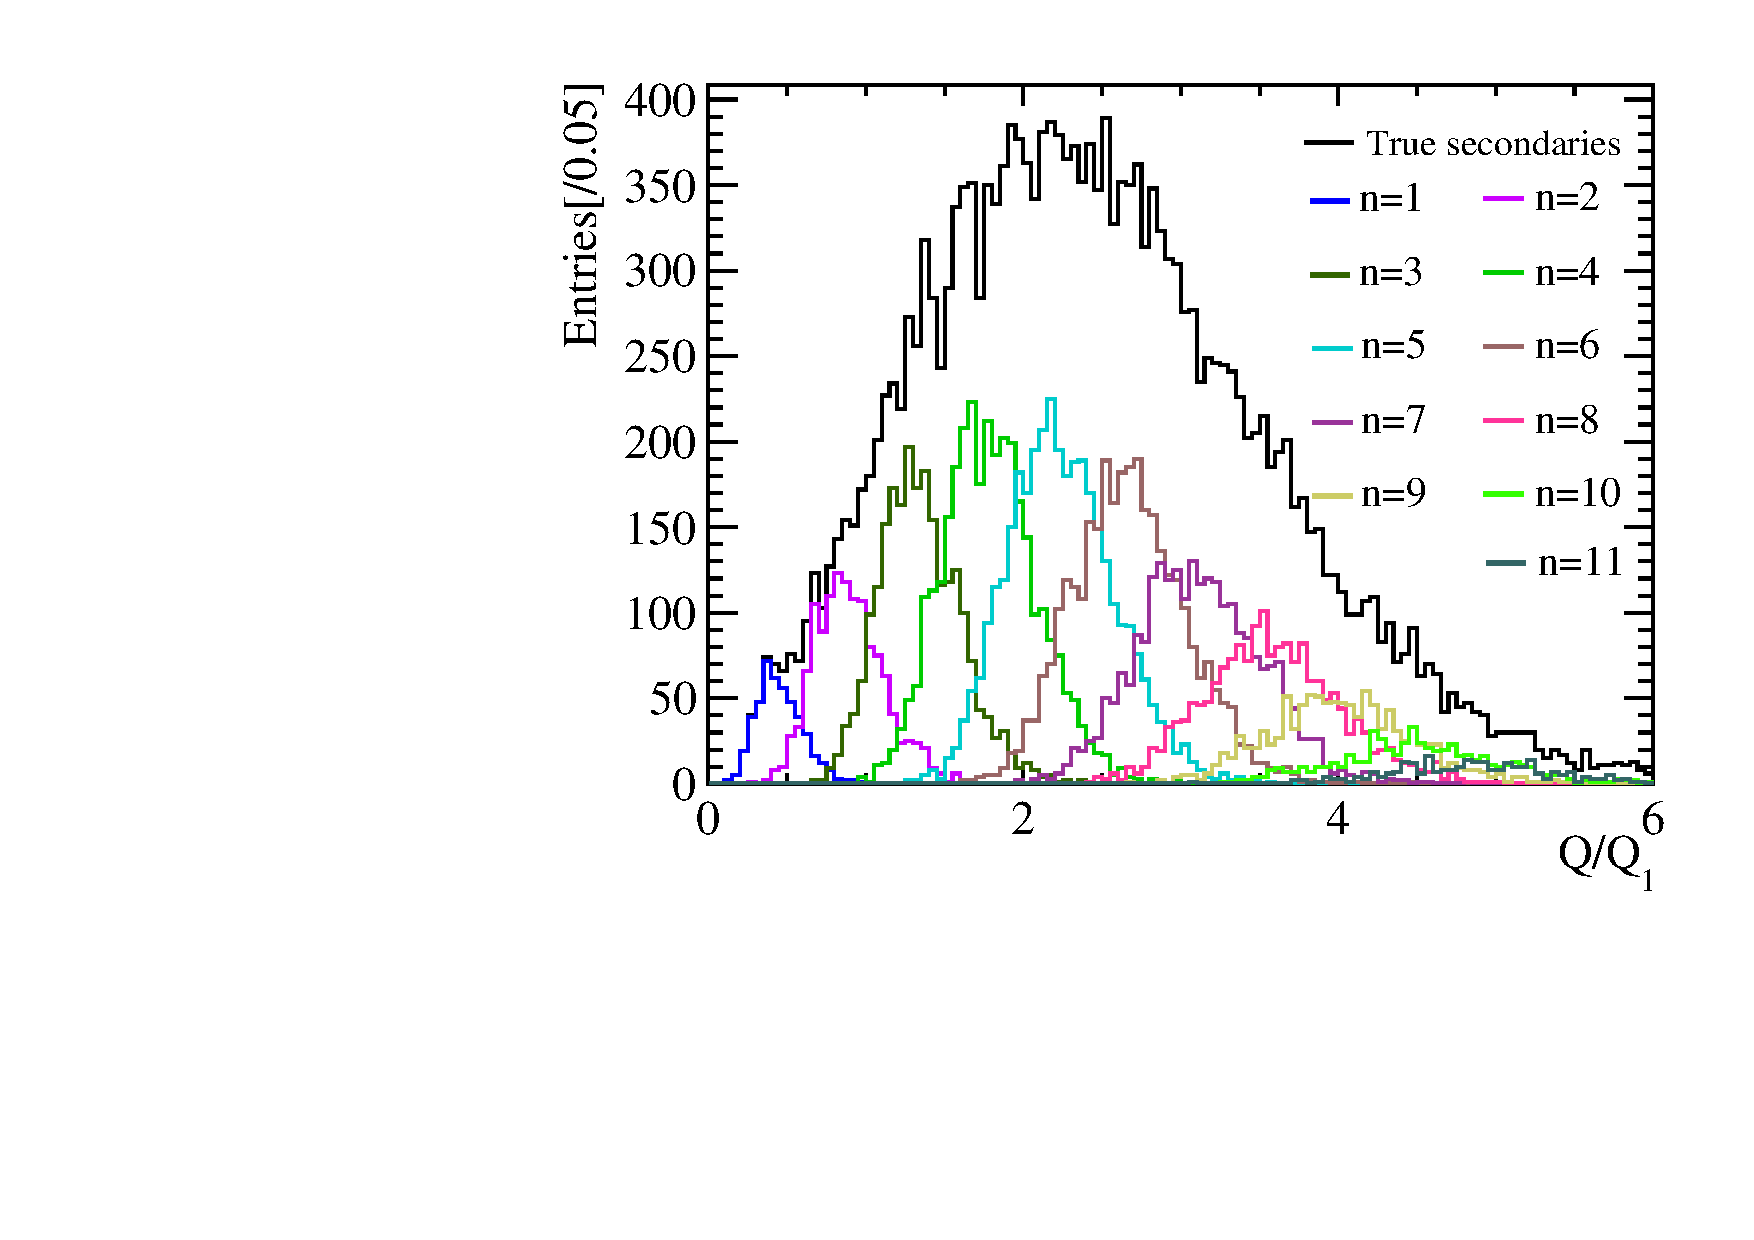
\includegraphics[width=\textwidth]{PMTRelated/GTmodel/true_all.pdf}
		\caption{}
		\label{fig:true_n}
	\end{subfigure}
	\hfill
	\begin{subfigure}{0.47\linewidth}
		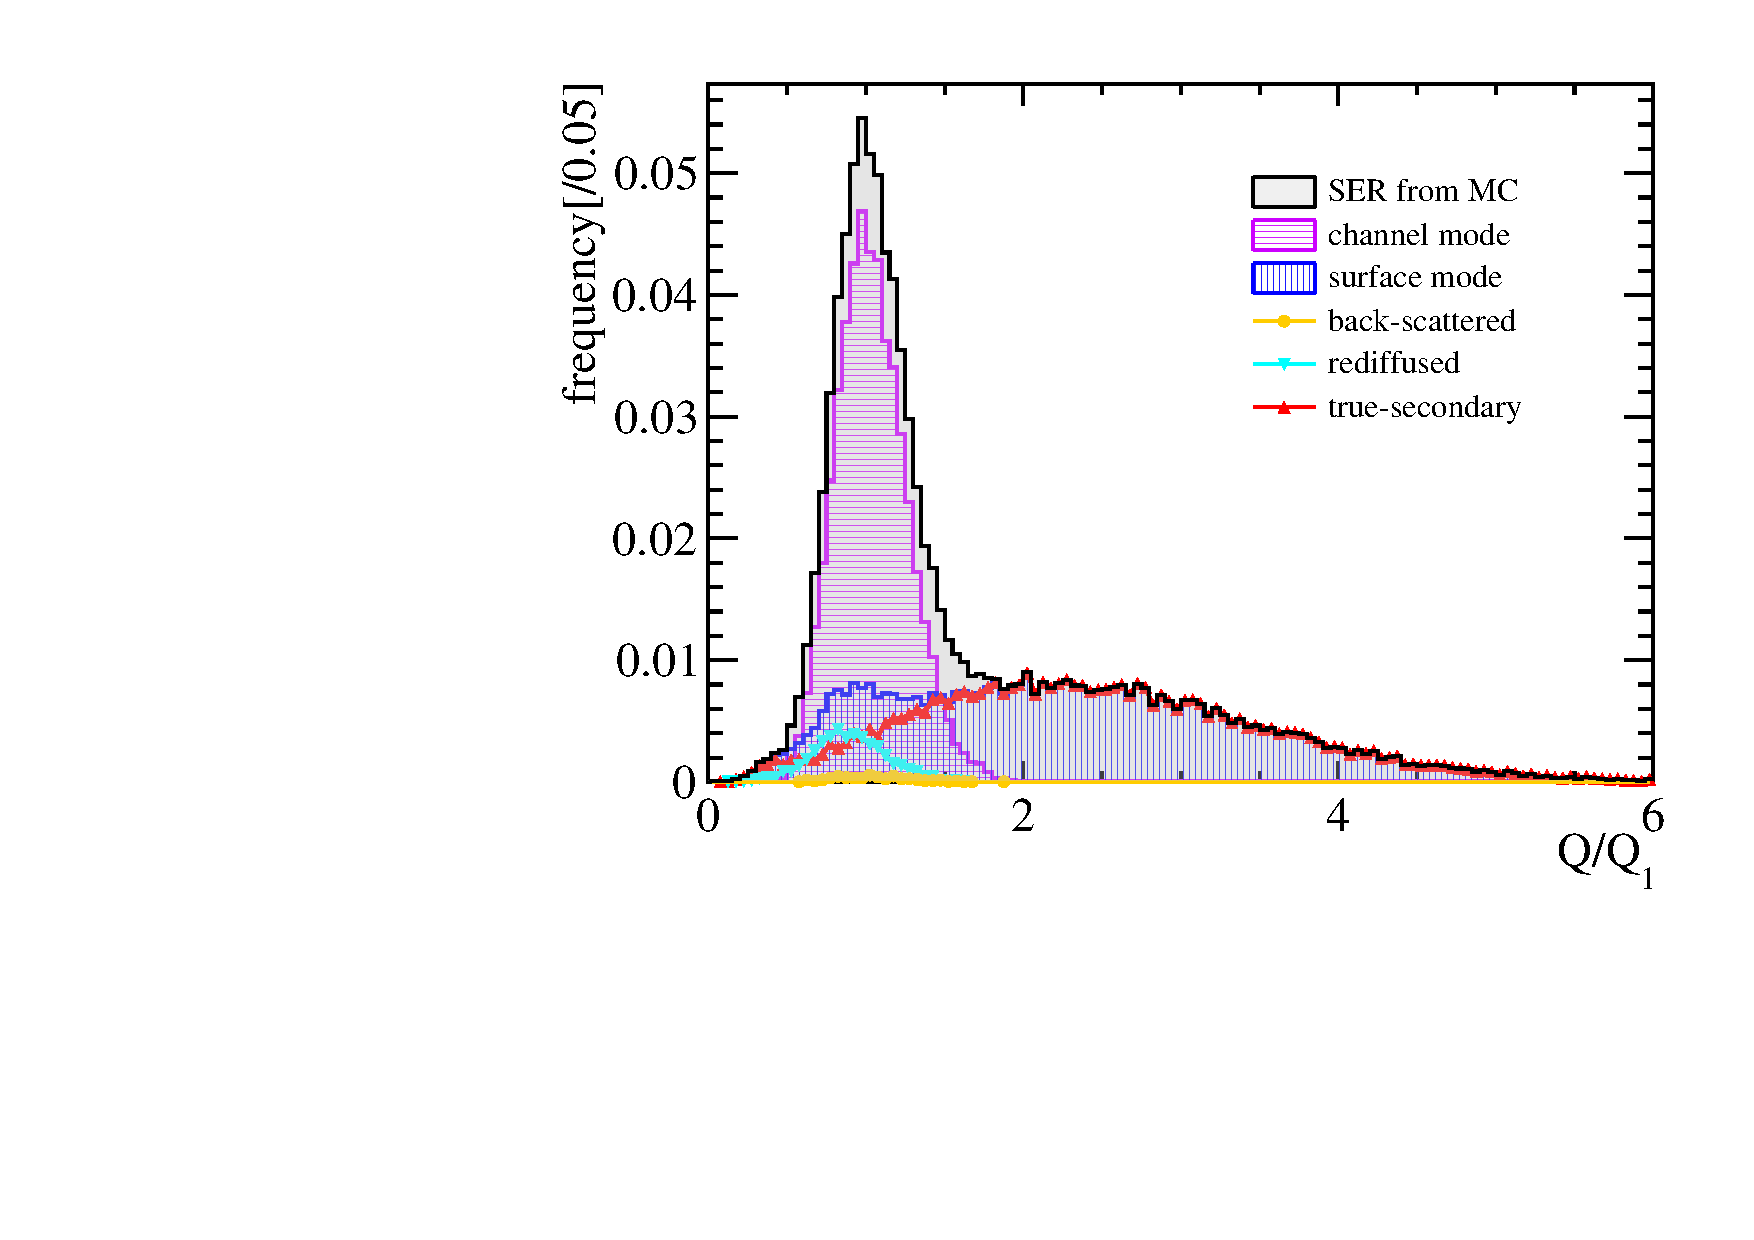
\includegraphics[width=\textwidth]{PMTRelated/GTmodel/allmode.pdf}
		\caption{}
		\label{fig:allmode}
	\end{subfigure}
	\caption{\subref{fig:true_n}: The charge distribution of the true-secondary electrons mode
		in the MC calculation when $\delta_{\mathrm{ts}}'=5.5$ and $p_0=0.55$.
		The black histogram gives the sum of all the distributions.
		\subref{fig:allmode}: The charge distribution formed in the channel mode is concentrated around the peak,
		while the tail portion is mainly generated by the true-secondary electrons in the surface mode.}
\end{figure}

A typical decomposition of the SER charge spectra is shown in Fig.~\ref{fig:allmode}.
The jumbo charges, also known as the ``long tail'', are contributed by the true secondaries
from the surface mode.

\subsection{Parameter Extraction from Data}\label{subsec:chitest}
It is evident from Eq.~(\ref{eq:1}) and (\ref{eq:ts_all}) that $\delta_{\mathrm{ts}}'$ and \(p_0\)
significantly impact the SER charge distribution, demonstrated in Fig.~\ref{fig:tsp}.  We use
the MCP-PMT test data by Zhang~et~al.~\cite{Zhang:2023ued} to determine the two parameters.
\begin{figure}[!htbp]
	\centering
	\begin{subfigure}{0.47\textwidth}
		\centering
		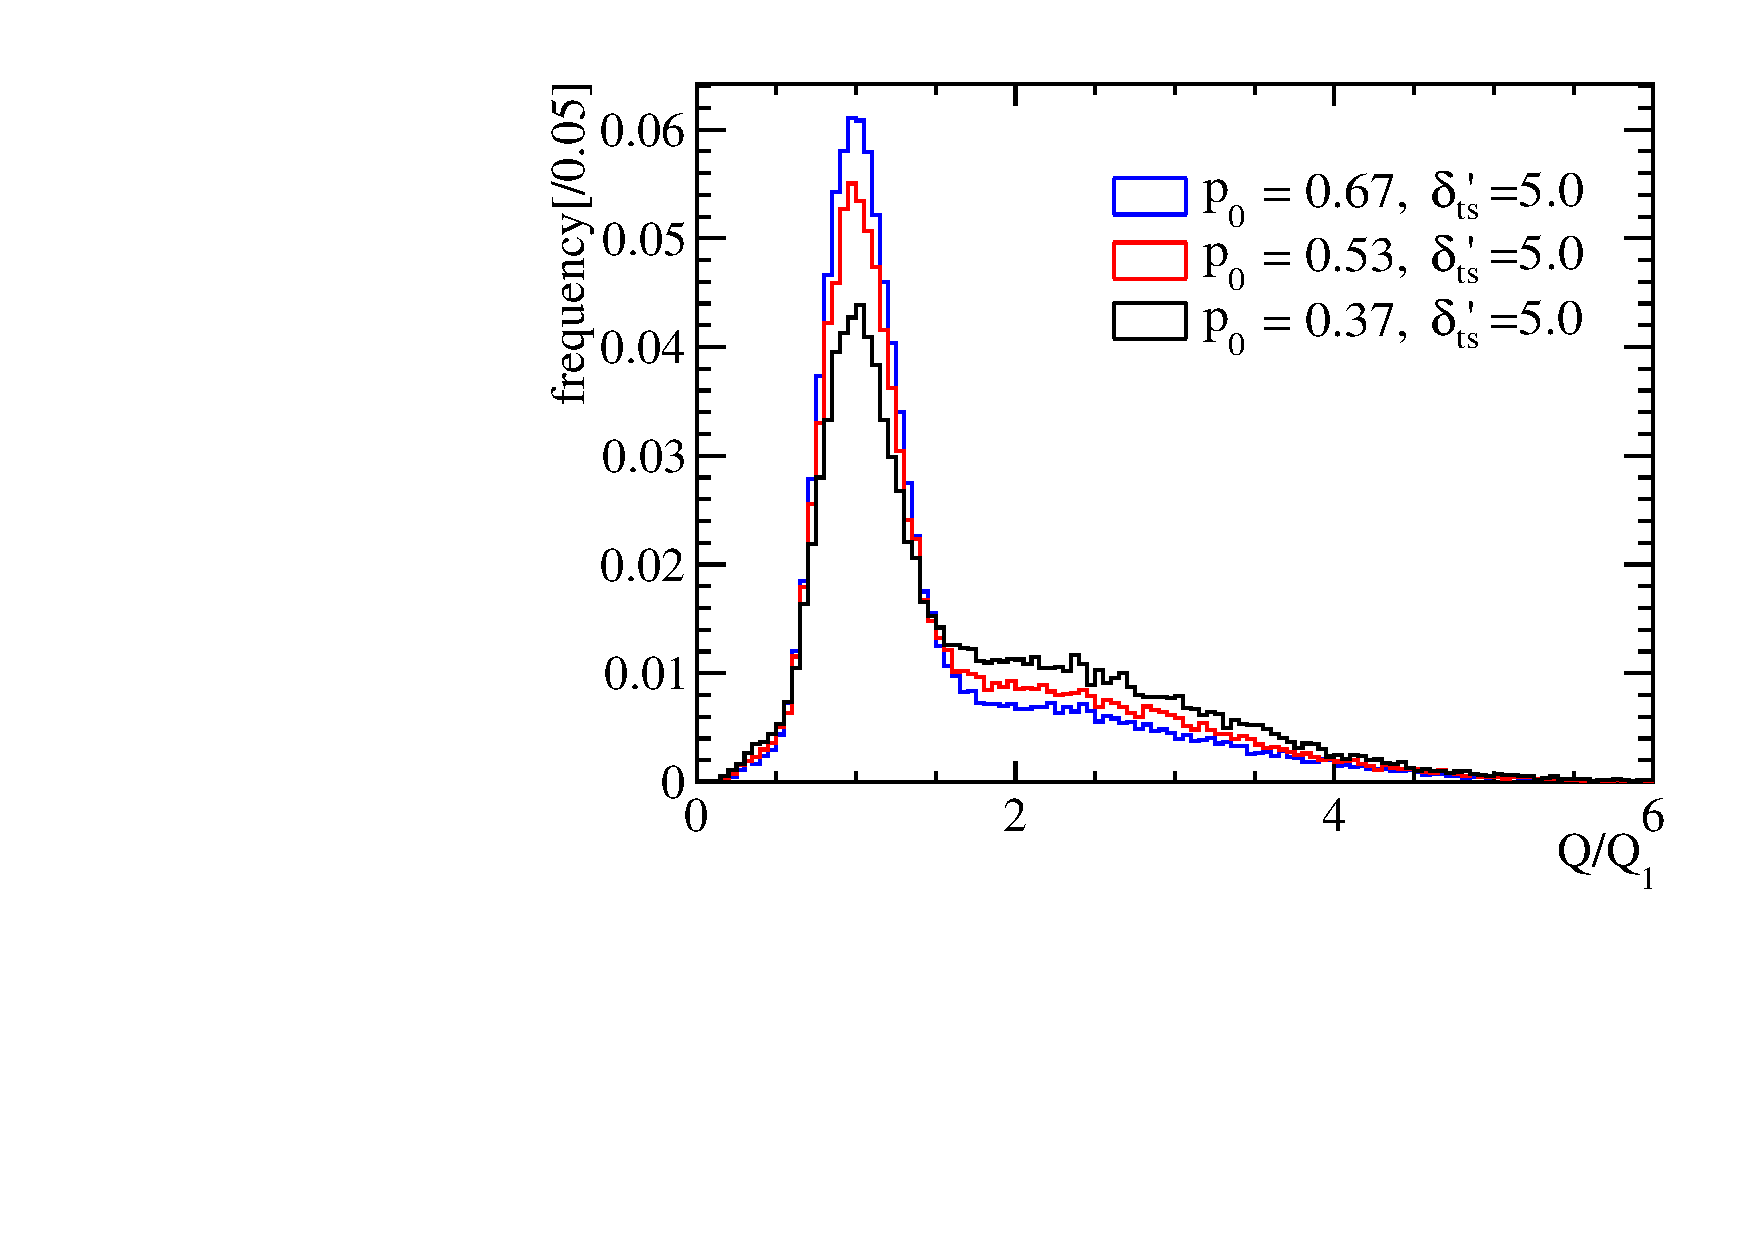
\includegraphics[width=\linewidth]{PMTRelated/GTmodel/p.pdf}
		\caption{}
		\label{fig:p}
	\end{subfigure}
	\hfill
	\begin{subfigure}{0.47\textwidth}
		\centering
		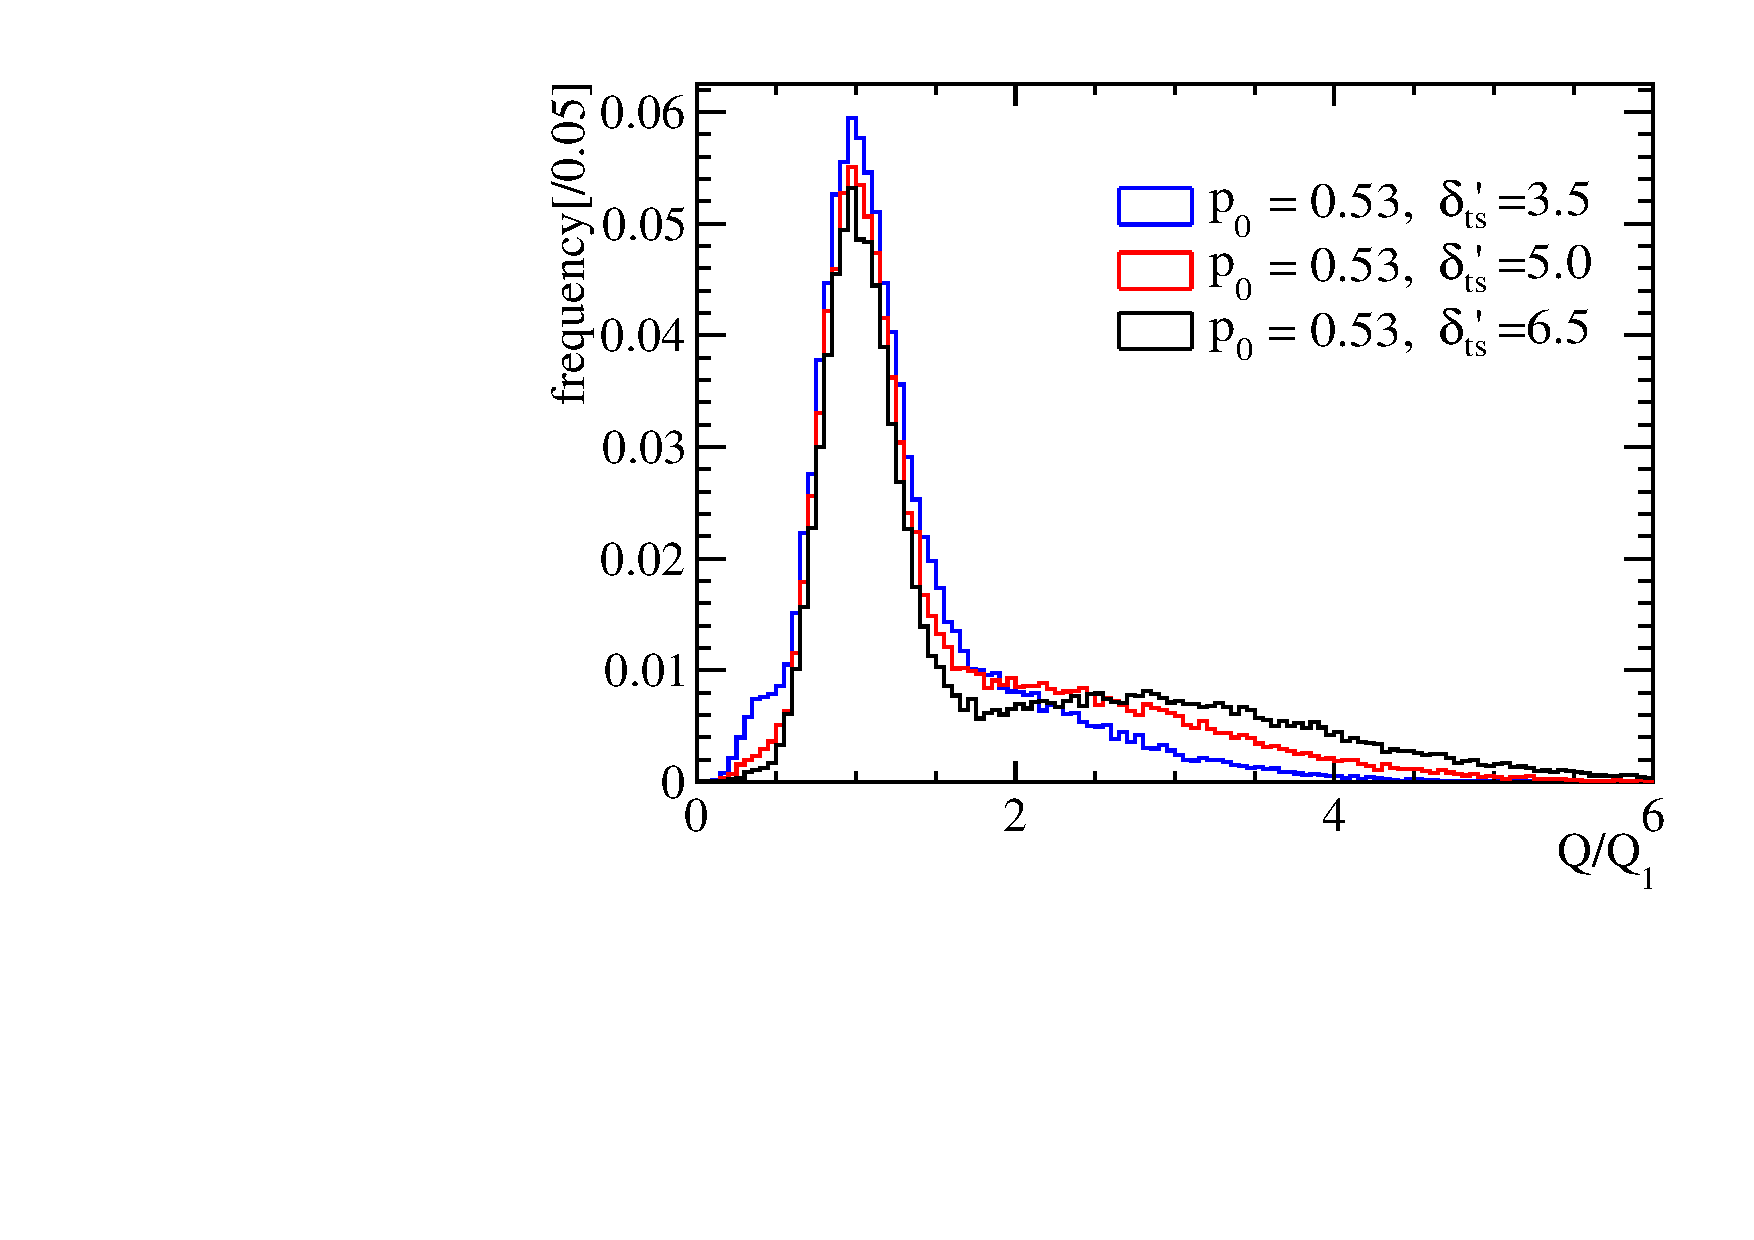
\includegraphics[width=\linewidth]{PMTRelated/GTmodel/ts.pdf}
		\caption{}
		\label{fig:ts}
	\end{subfigure}
	\caption{$\delta_{\mathrm{ts}}'$ and $p_0$ influence the shape of SER charge spectrum from MC.
		As $\delta_{\mathrm{ts}}'$ increases, the region of the tail becomes more prolonged.
		As $p_0$ increases, the height of the principal peak region increases, and the tail becomes narrower.
	}
	\label{fig:tsp}
\end{figure}

Between each pair of predicted and measured charge distributions, we perform a chi-square test.
These two histograms are divided into $r$ bins using the same binning method.
The entries in the \(i\)-th bin are $n_i$ and $m_{i}$, adding up to
$N = \sum_{{i}=1}^{r}n_{i}$ and $M = \sum_{{i}=1}^{r}m_{i}$.
The chi-square test indicates the similarity between two histograms~\cite{2006Comparison},
\begin{equation}
	\label{eq:chi}
	\chi^2_{r-1}=\sum_{{i}=1}^r \frac{\left(n_{i}-N \hat{k}_{i}\right)^2}{N \hat{k}_{i}}+\sum_{{i}=1}^r
	\frac{\left(m_{i}-M \hat{k}_{i}\right)^2}{M \hat{k}_{i}}=\frac{1}{M N} \sum_{{i}=1}^r
	\frac{\left(M n_{i}-N m_{i}\right)^2}{n_{i}+m_{i}}
\end{equation}
where \(\hat{k}_{i}=\frac{n_{i}+m_{i}}{N+M}\).

The \(\chi^2_{r-1}\) are scanned in the $(p_0,\delta_{\mathrm{ts}}')$ grid, with an example in Fig.~\ref{fig:cour}.
We use a linear model~\cite{Gelman_Hill_2006} to smooth the approximate parabolic relationship
between the \(\chi^2_{r-1}\) and $(p_0, \delta_{\mathrm{ts}}')$,
then extract the $(\hat{p}_0, \hat{\delta}_{\mathrm{ts}}')$ that minimizes \(\chi^2_{r-1}\) with
intervals at \SI{68.3}{\percent} confidence levels~\cite{cowan1997statistical}.

\begin{figure}[!htbp]
	\centering
	\begin{subfigure}{0.47\textwidth}
		\centering
		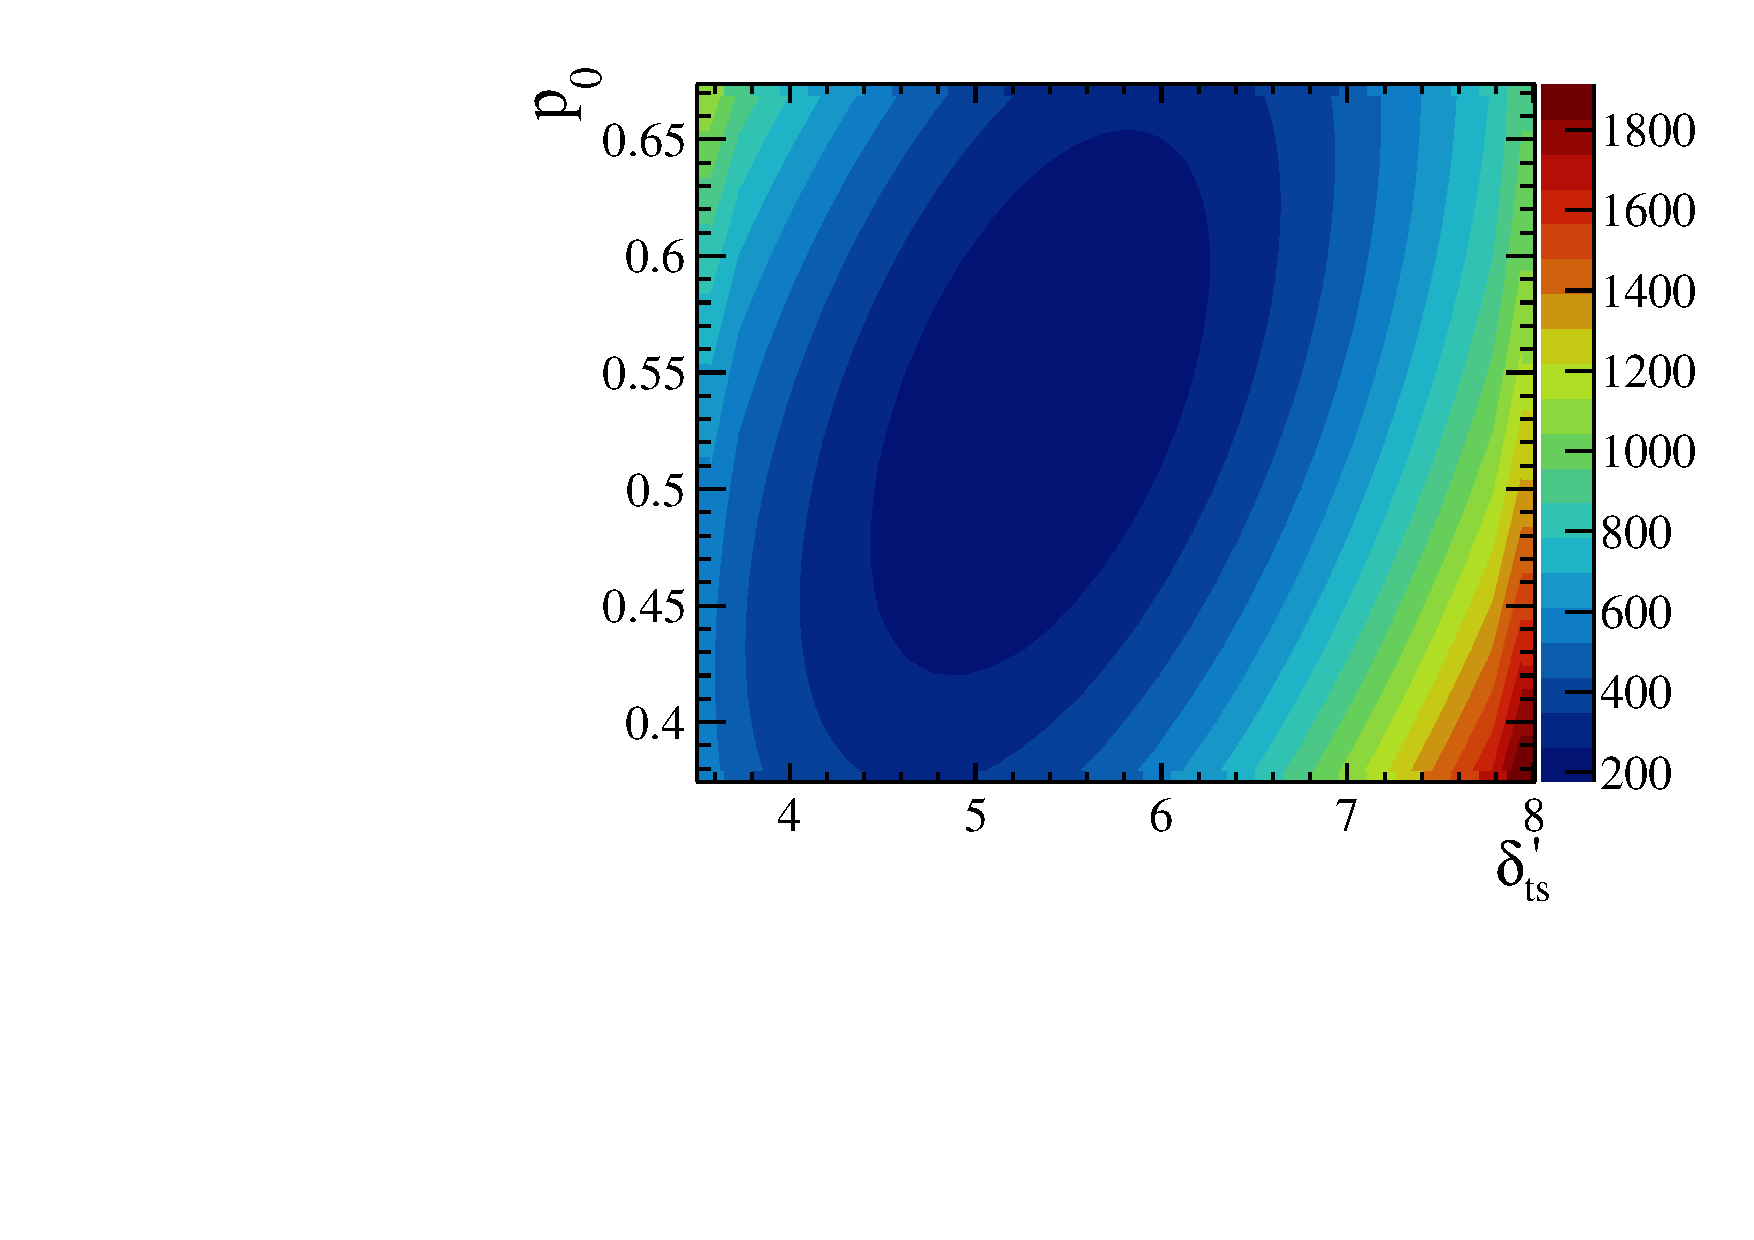
\includegraphics[width=\linewidth]{PMTRelated/GTmodel/cour.pdf}
		\caption{}
		\label{fig:cour}
	\end{subfigure}
	\hfill
	\begin{subfigure}{0.47\textwidth}
		\centering
		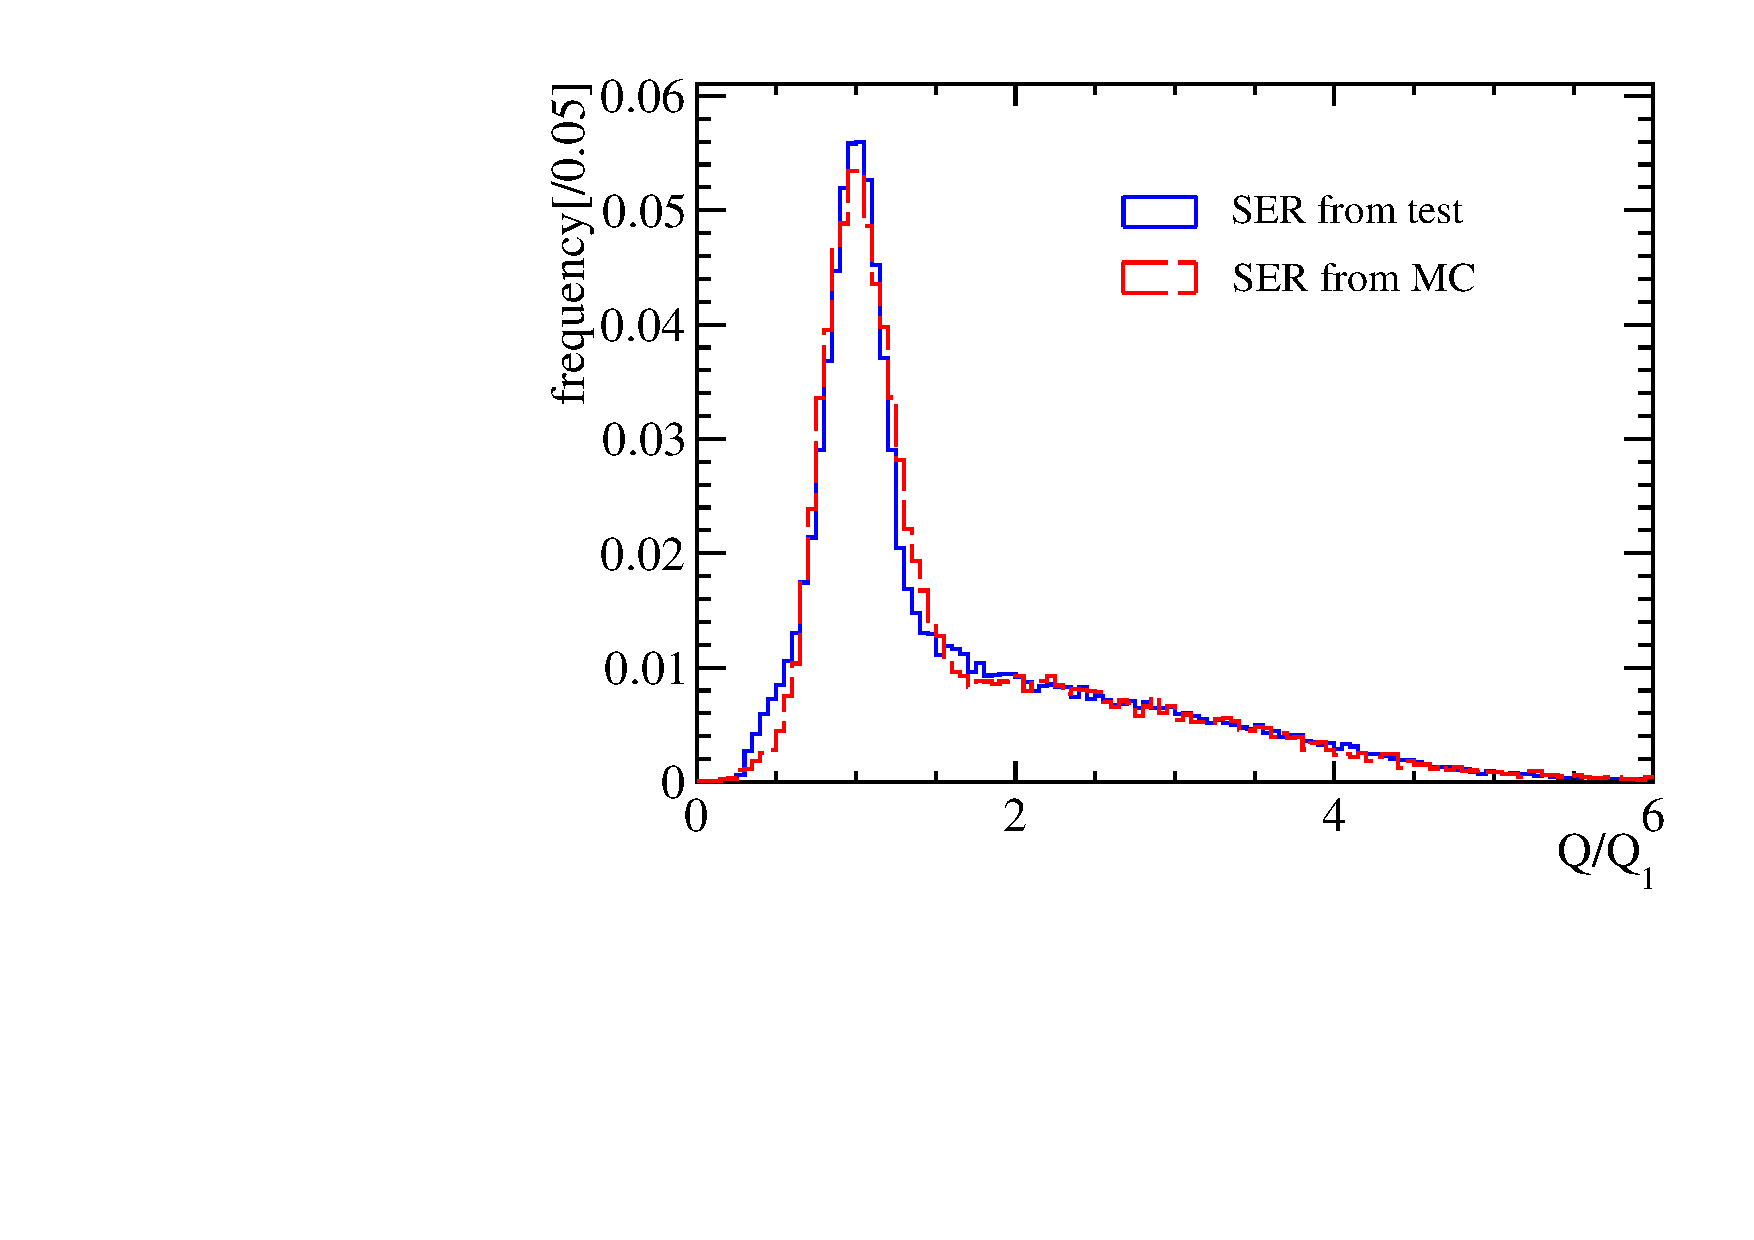
\includegraphics[width=\linewidth]{PMTRelated/GTmodel/hist.pdf}
		\caption{}
		\label{fig:hist}
	\end{subfigure}
	\caption{The plot~\subref{fig:cour} is the contour plot of the chi-square test, with $p_0$ and $\delta_{\mathrm{ts}}'$ as parameters
		and the chi-square values as the height.
		The plot~\subref{fig:hist} is an example of the MC histogram~(the red line) and the histogram from test~(the blue line).
	}
	\label{fig:chi}
\end{figure}

The $\hat{\delta}_{\mathrm{ts}}'$ vs. $\hat{p}_0$ scatter plot
of 9 MCP-PMTs in Fig.~\ref{fig:true_p} does not indicate a strong correlation.
They are determined by independent manufacturing stages.
On average, $\delta_{\mathrm{ts}}'$ is 5.979 and $p_0$ is 0.5341. % rd=0.09,bs=0.01
The PEs of the channel, back-scattered, and rediffused surface modes account for \SI{53.41}{\percent}.
They constitute the peak. Each of the rest hits the surface
to induce 5.979 true-secondary electrons on average.

\begin{figure}[!htbp]
	\centering
	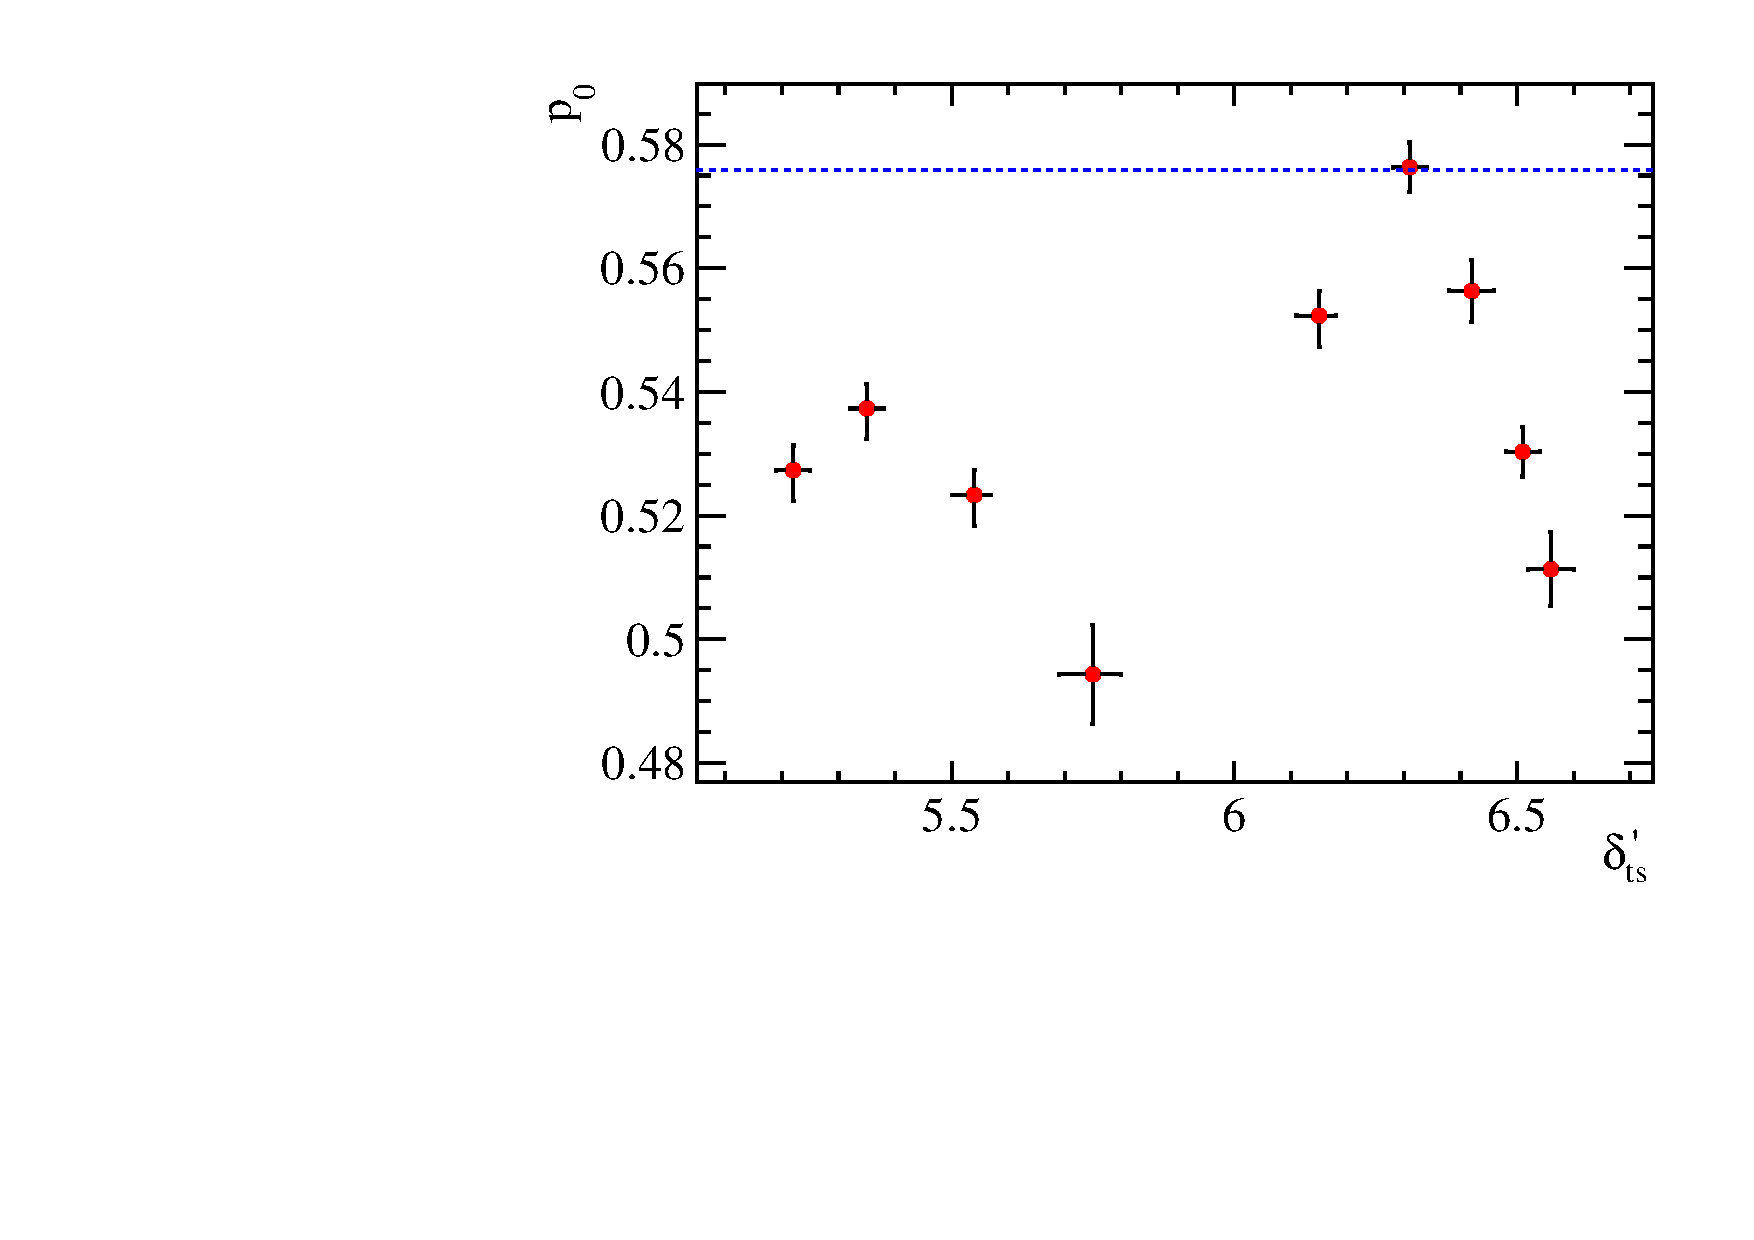
\includegraphics[width=0.6\textwidth]{PMTRelated/GTmodel/true_p.pdf}
	\caption{When convolving with 9 MCP-PMTs,
		the distribution of $\delta_{\mathrm{ts}}'$ and $p_0$ at the minimum chi-square
		occurs. The blue dashed line shows the expected $\hat{p}_0$ estimated from~\cite{chen2018photoelectron}.}
	\label{fig:true_p}
\end{figure}

To compare our measurement to previous studies, we convert \(\delta_\text{ts}'\)
to the SEY \(\delta\)
\begin{equation}
	\label{eq:2}
	\delta = \delta_\text{bs} + \delta_\text{rd} + (1-\delta_\text{bs} - \delta_\text{rd}) \delta_\text{ts}'
\end{equation}
and the fraction \(p_0\) to \(p\) by Eq.~\eqref{eq:p0}.
Cao~et~al.\cite{cao_secondary_2021} measured the SEY of \ce{Al2O3}-\ce{MgO} double-layered film
to be 4--5. Chen~et~al.~\cite{2016Optimization} pointed out
that there is an electrostatic lens effect at the MCP channel entrances,
making the ratio of the PEs entering the MCP channels
smaller than the open-area ratio.
When PEs come with an incident angle~$\theta_0=0^\circ$,
the proportion of the PEs directly entering the MCP channels is around \SI{60}{\percent} when the MCP open-area ratio is \SI{74.9}{\percent}.
Chen~et~al.~\cite{chen2018photoelectron} indicated that
the proportion is around \SI{55}{\percent} when the open-area ratio is \SI{65}{\percent}.
The MCPs in our case have pore diameters of \SI{12}{\mu\meter}, spacings of \SI{14}{\mu\meter} between the pores,
and open-area ratios of \SI{66.6}{\percent}.
The expected $\hat{p}_0 = \frac{55\%}{1-(1-55\%)(\delta_{\mathrm{rd}}+\delta_{\mathrm{bs}})}\approx 57.6\%$ for $\delta_{\mathrm{rd}}+\delta_{\mathrm{bs}}=0.1$.
\begin{figure}[!htbp]
	\centering
	\begin{subfigure}{0.48\textwidth}
		\centering
		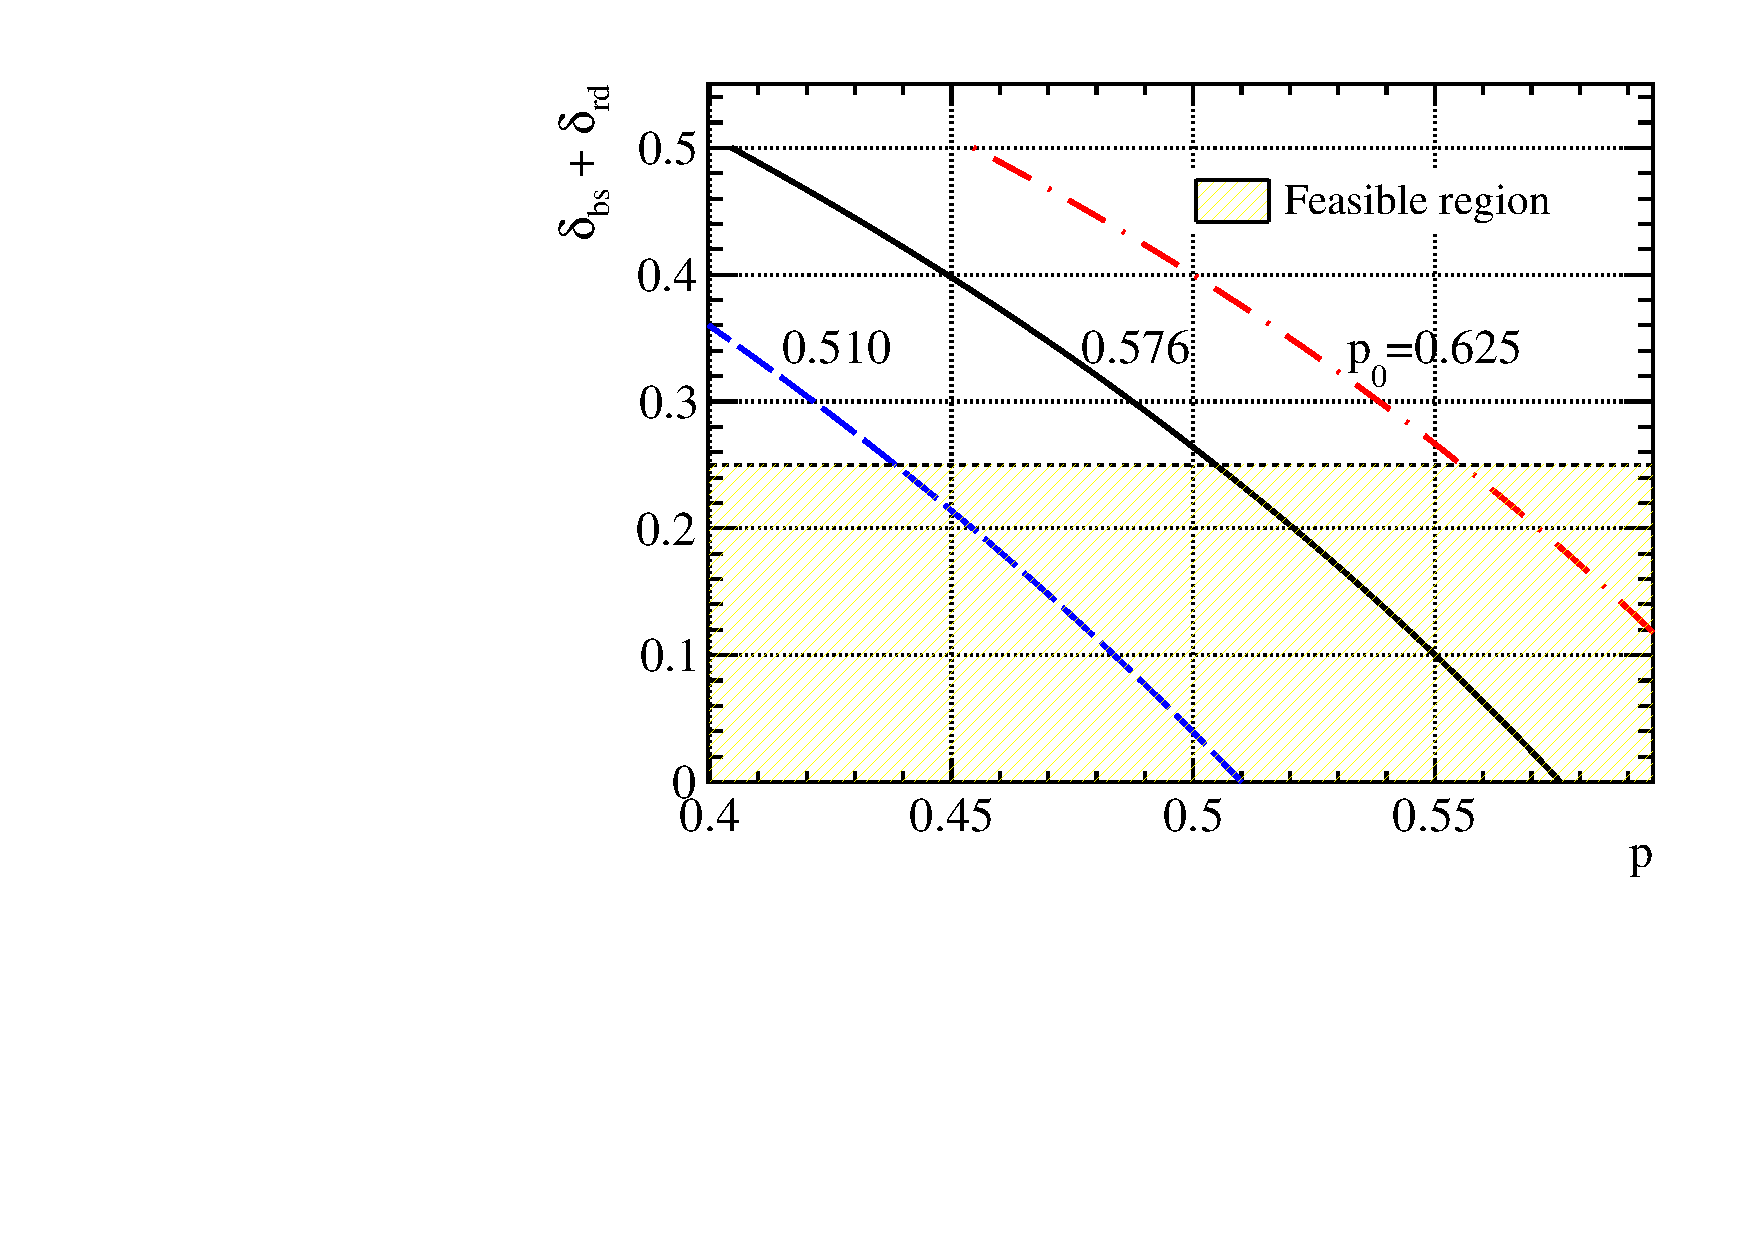
\includegraphics[width=\linewidth]{PMTRelated/GTmodel/parameter_pp0.pdf}
		\caption{}
		\label{fig:pp0}
	\end{subfigure}
	\hfill
	\begin{subfigure}{0.48\textwidth}
		\centering
		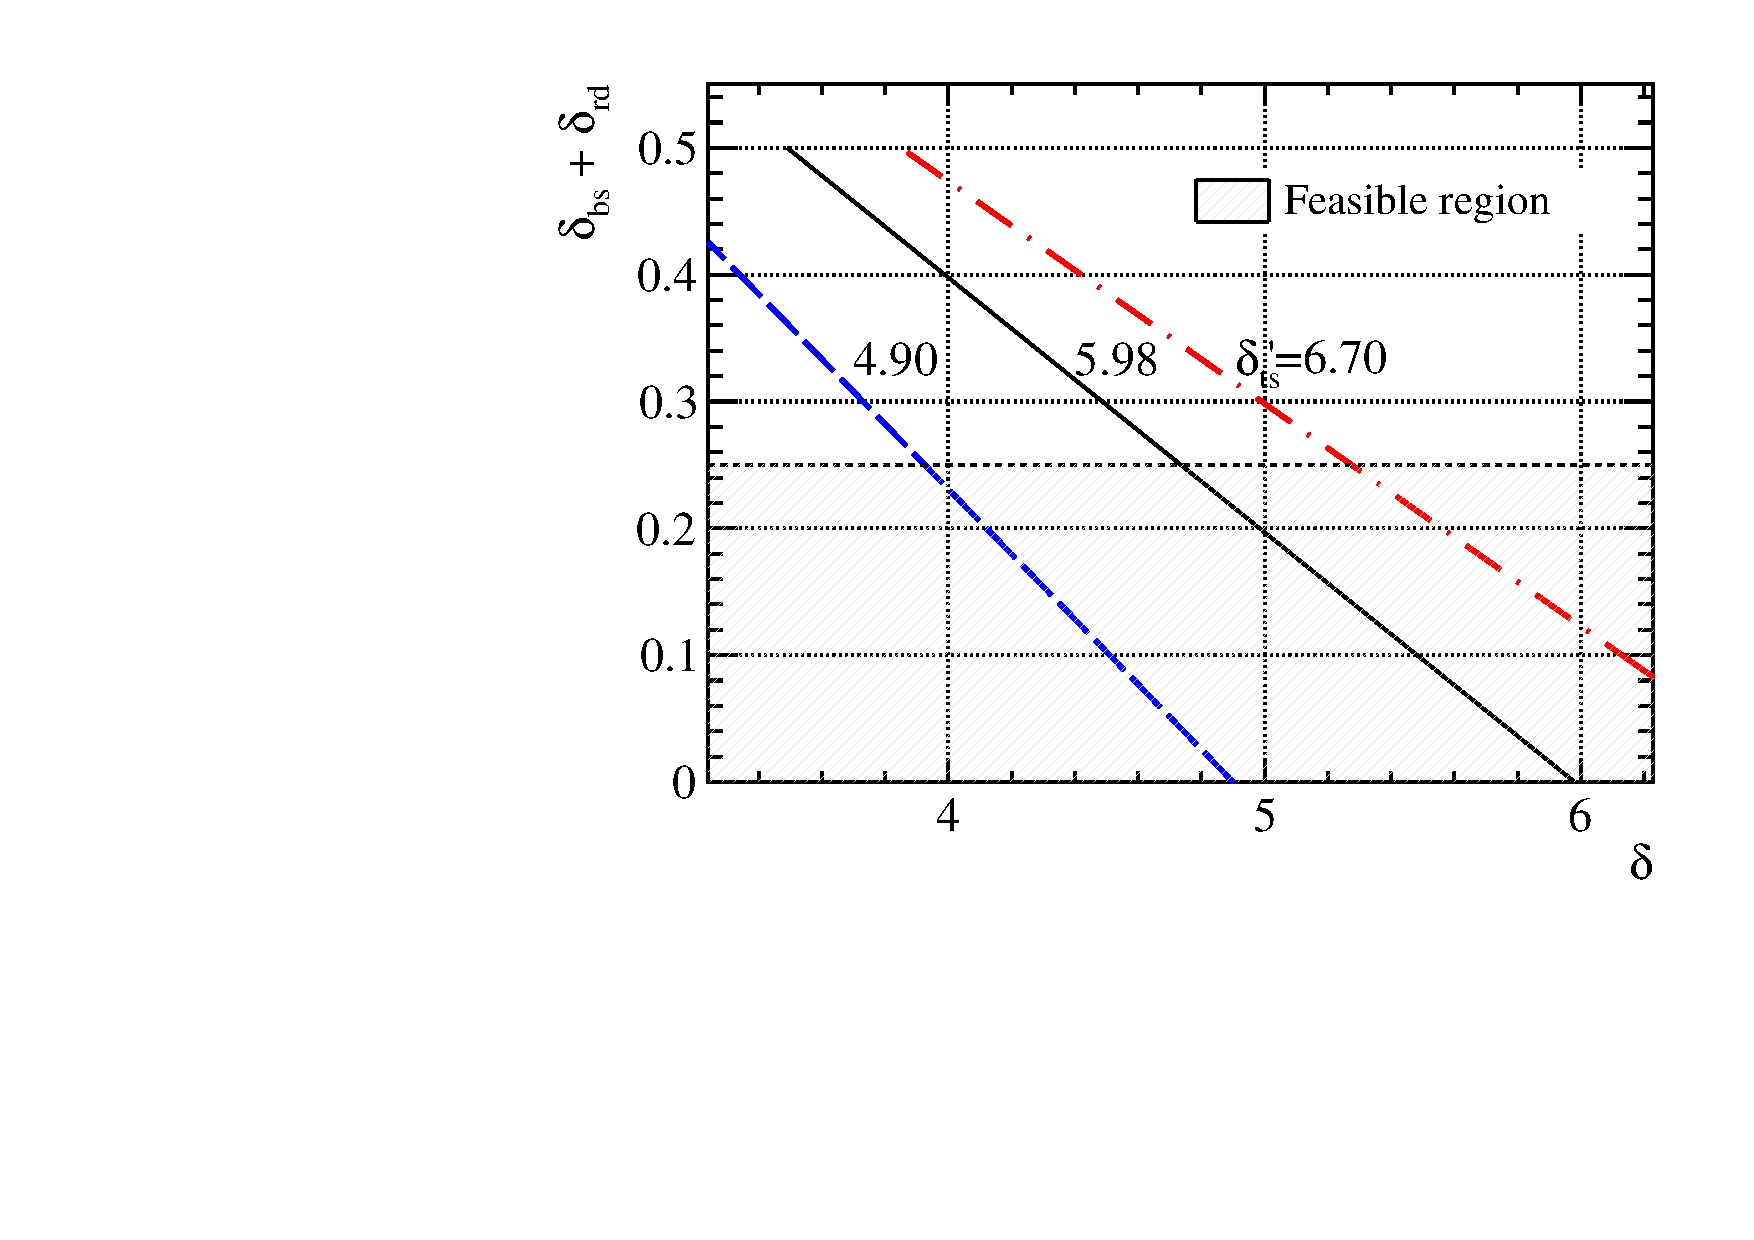
\includegraphics[width=\linewidth]{PMTRelated/GTmodel/parameters_ts.pdf}
		\caption{}
		\label{fig:tsts}
	\end{subfigure}
	\caption{Relations of \(\delta_\text{bs} + \delta_\text{rd}\) against the SEY \(\delta\) and the fraction of channel mode \(p\).
		The feasible region shows the consistency of our measurement to the literature.}
	\label{fig:pdelta}
\end{figure}

In Fig.~\ref{fig:pdelta}, with the typical values of \(\delta=5\) and \(p=0.55\),
our measurement is consistent with an assumption that \(\delta_\text{bs} + \delta_\text{rd} < 0.25\).
The small contribution of the back-scattered and rediffused electrons in SEE is pointed out by Beck~\cite{beck_physical_1966} to be especially true for insulators with high SEY.


\subsection{Gamma-Tweedie model for MCP-PMT}\label{sec:model}
In our calculation, the distribution of the MCP charge response to the true-secondary electrons $\varGamma(\alpha_{i},\beta_{i})$ is determined by their energies $E_{i}$,
which satisfy $\sum_{i}^{n}E_{i}<E_0$.
The incident energy \(E_0\) of the PEs is \SI{650}{eV},
which is more than ten times the energies of the true secondaries.
Because $n$ follows a Poisson distribution with an expectation between 5 and 6.5,
the probability of $n$ exceeding 10 is negligible.
Thus, the effect of $n$ on $E_{i}$ can be ignored,
and the energy \(E_{i}\) is independently and identically distributed, as demonstrated in Fig.~\ref{fig:single_pe}.
The charge response of MCP to a single true-secondary electron, in turn, can be treated identically, as shown in Fig.~\ref{fig:single_fit}.
Furthermore, a single Gamma distribution \(\varGamma(\alpha',\beta')\)
is flexible enough to describe the continuous mixture of
\(\int dE_{i}\frac{1}{\delta_{\mathrm{ts}}}\frac{d\delta_{\mathrm{ts}}}{dE_{i}}\varGamma[\alpha(E_{i}),\beta(E_{i})]\).

\begin{figure}[!htbp]
	\centering
	\begin{subfigure}{0.47\textwidth}
		\centering
		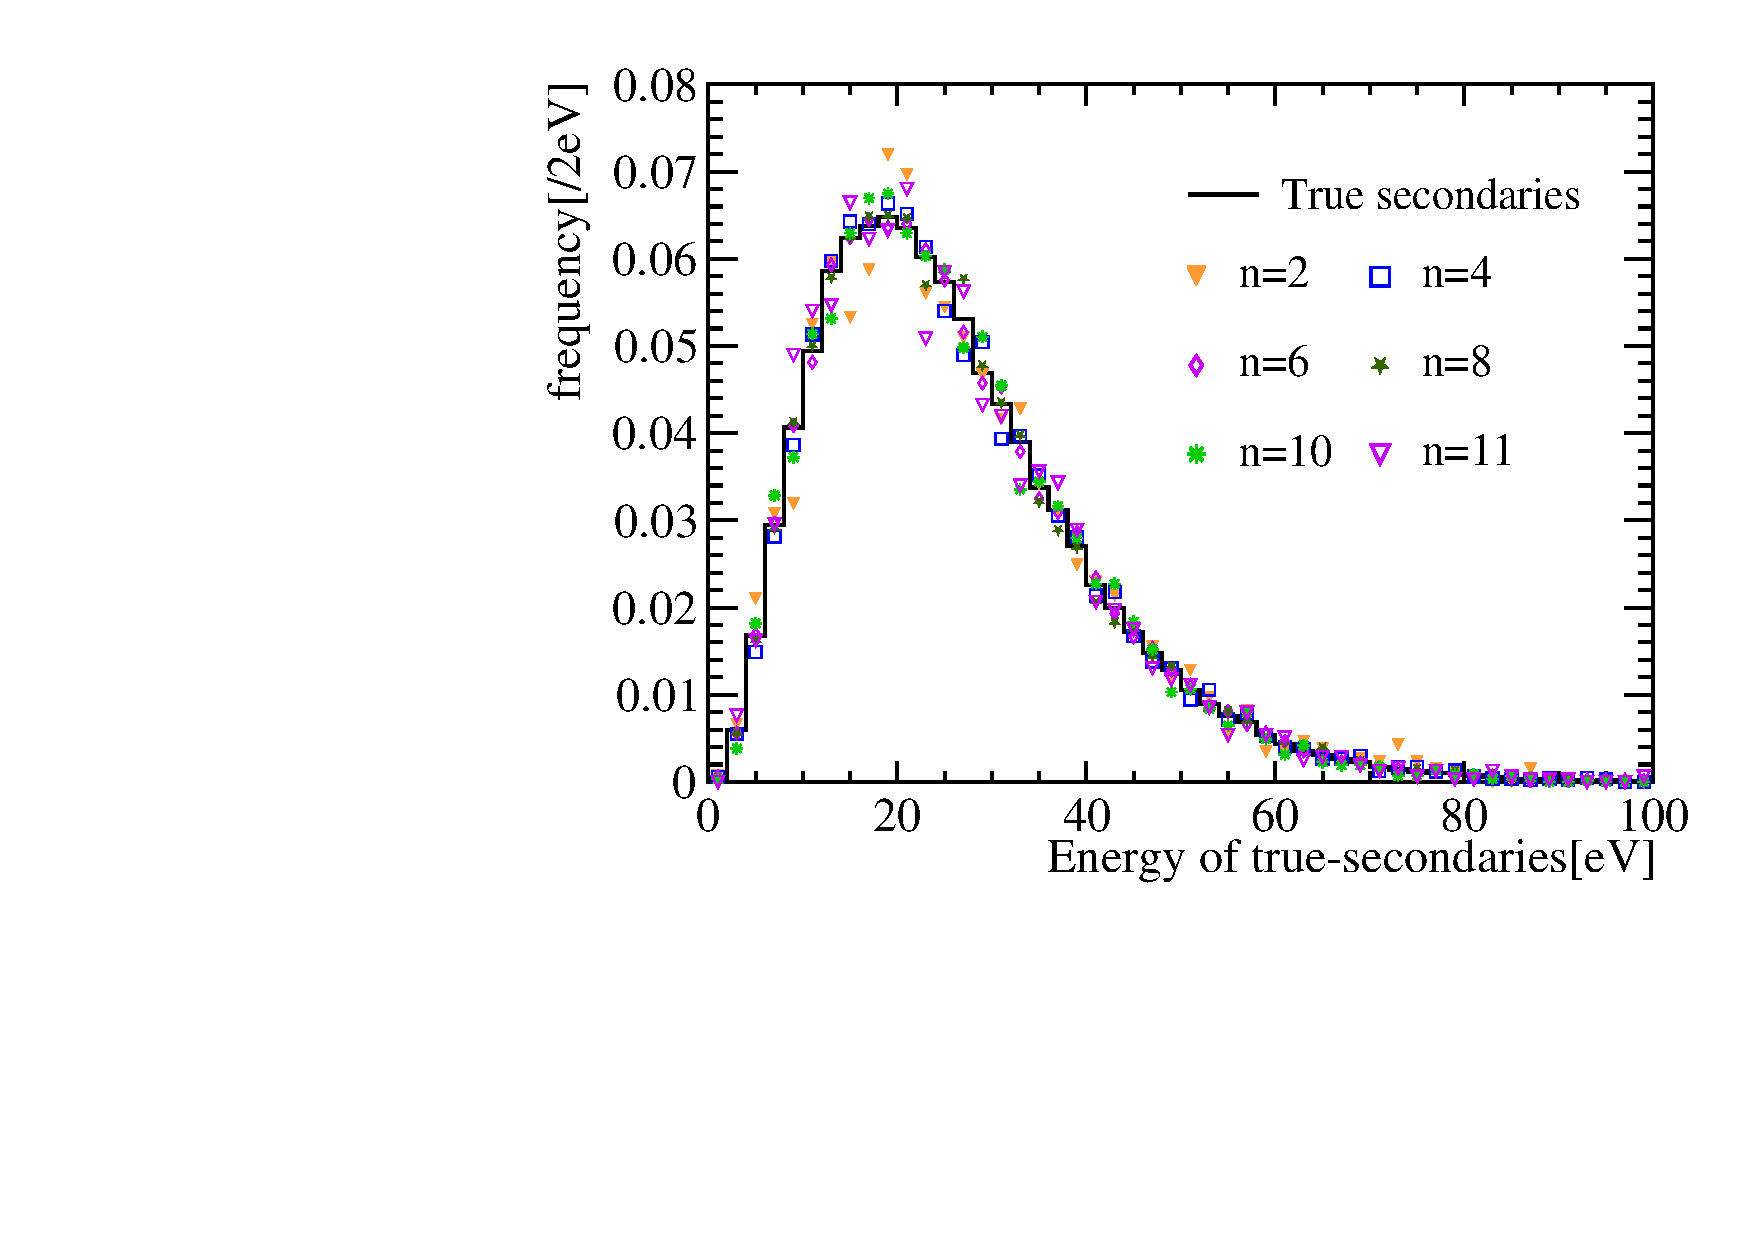
\includegraphics[width=\linewidth]{PMTRelated/GTmodel/single_pecharge.pdf}
		\caption{}
		\label{fig:single_pe}
	\end{subfigure}
	\hfill
	\begin{subfigure}{0.47\textwidth}
		\centering
		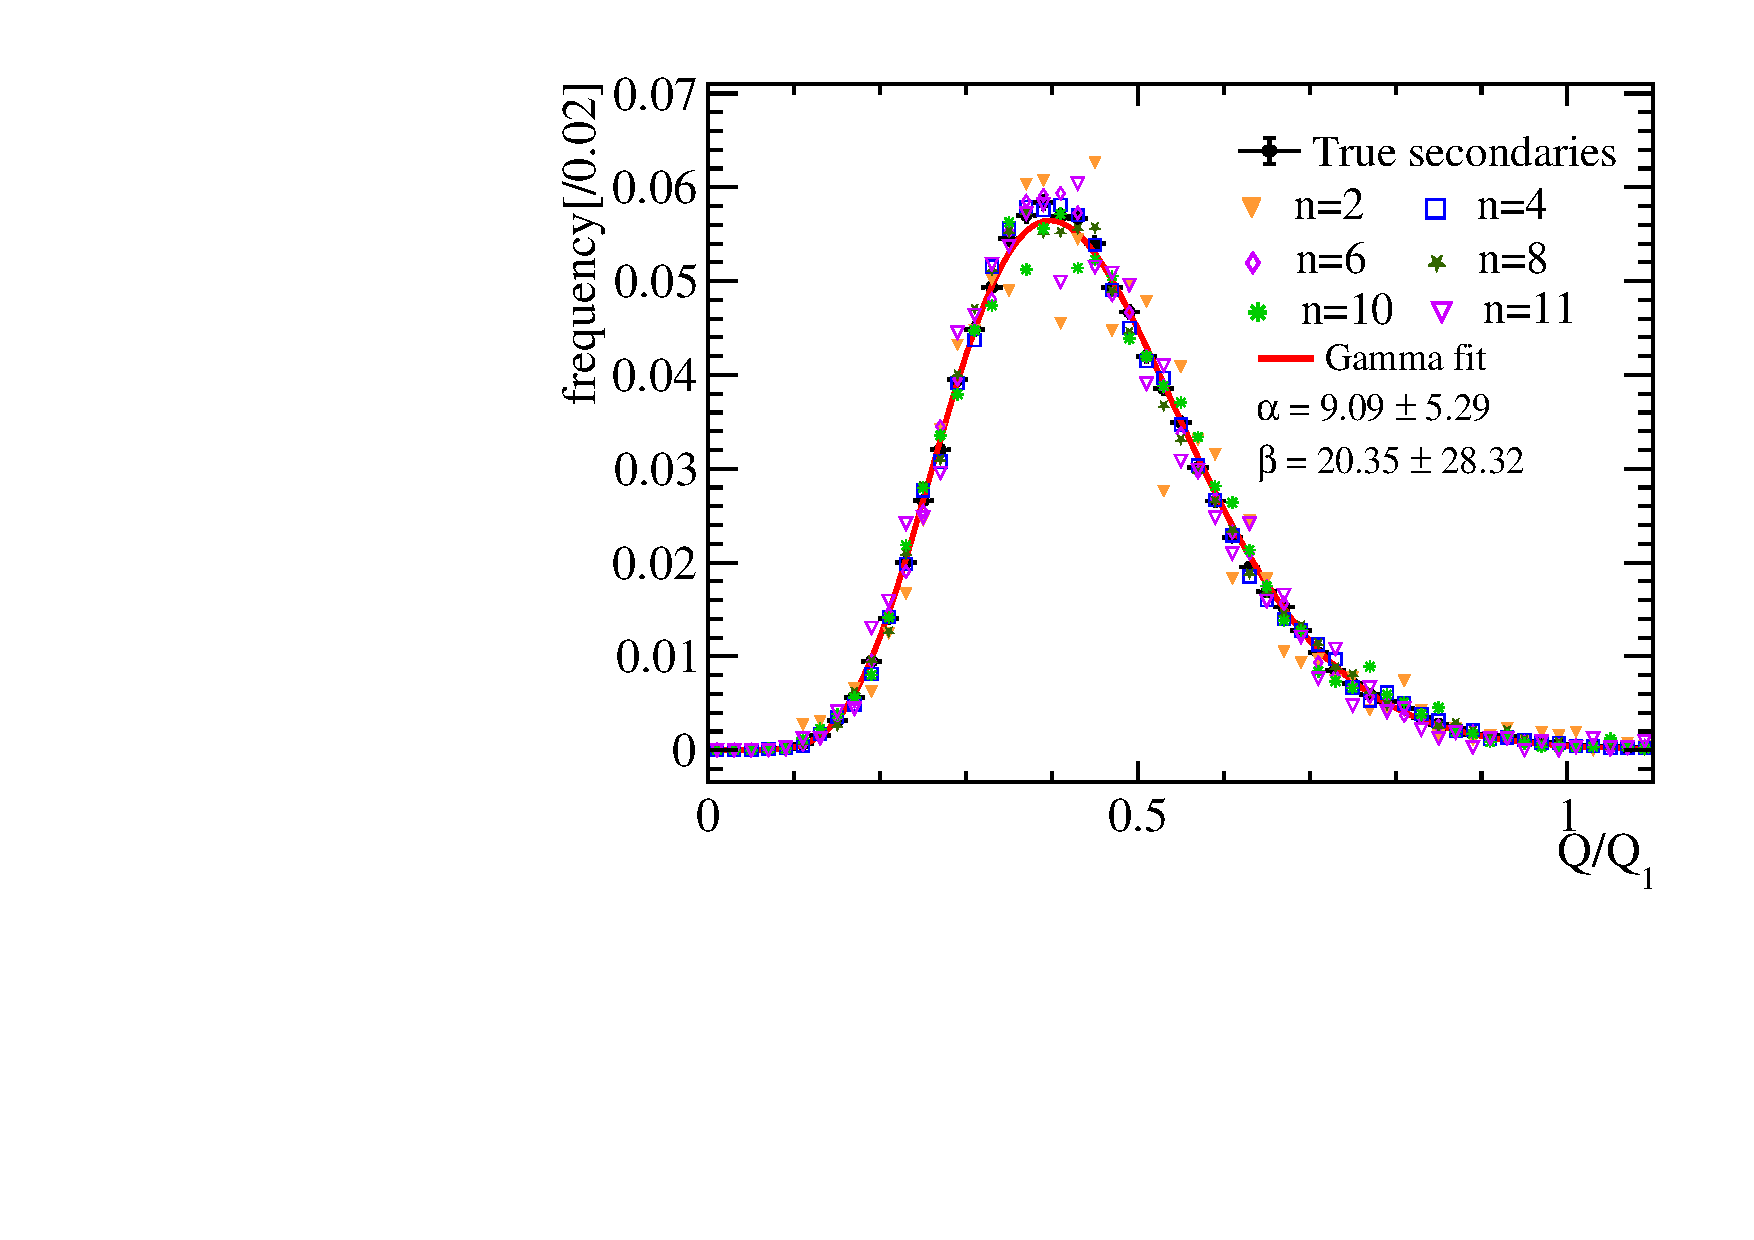
\includegraphics[width=\linewidth]{PMTRelated/GTmodel/singlepefit.pdf}
		\caption{}
		\label{fig:single_fit}
	\end{subfigure}
	\caption{The energy distribution and the charge response distribution of MCP to a single true-secondary electron when $n$ is different.
		\subref{fig:single_pe}: All the energies of the true secondaries follow the same distribution,
		although $n$ is different.
		\subref{fig:single_fit}: the charge response of MCP to a single true-secondary electron is identical,
		and the fitting of the Gamma distribution~\(\varGamma(\alpha',\beta')\)
		achieves sufficient goodness.}
	\label{fig:singlepe}
\end{figure}

When we use such a single \(\varGamma(\alpha', \beta')\) in Eq.\eqref{eq:ts_all},
the resulting Poisson-Gamma compound is a special case of the Tweedie distribution $\mathrm{Tw}_{\xi}(\alpha,\beta)$
for $1<\xi<2$~\cite{1991Tweedie}.
\begin{equation}
	\arraycolsep=1.4pt
	\label{eq:ts_gamma}
	\left.\begin{array}{rl}
		Q_{\text{ts}} & = \sum_{{i}=1}^{n} Q_{i}                 \\
		n             & \sim \mathrm{\pi}(\delta_{\mathrm{ts}}') \\
		Q_{i}         & \sim \varGamma(\alpha', \beta')
	\end{array}\right\} \implies
	Q_{\text{ts}} \sim \mathrm{Tw}_{\xi}(\alpha',\beta')
\end{equation}
A phenomenological joint fit of the \(f_\mathrm{ch}\) Gamma and \(f_\mathrm{ts}\) Tweedie
mixture with Eq.~\eqref{eq:1} and \eqref{eq:ts_gamma} is sufficient to calibrate the SER charge spectrum and measure \(p_0\) and \(\delta_\text{ts}'\).
The voltage division experiment~(Sec.~\ref{sec:gain}) relations \(\mu(E_i)\)/\(\sigma(E_i)\) and the Furman model provide the understanding of the jumbo charges and the justification of the phenomenological Gamma-Tweedie
mixture, but are less practically useful in PMT calibrations.

The number of parameters, 2 for \(f_\mathrm{ch}\) Gamma and 3 for \(f_\mathrm{ts}\) Tweedie,
hinders convergence unless we aid it with physical constraints.
Typically $\frac{\alpha'}{\beta'}\approx 0.45Q_1$ and \(\sqrt{\frac{\alpha'}{\beta'^2}}\approx 0.15Q_1\).
It is practical to bound them in $[0.3,0.7]Q_1$ and $[0.05,0.3]~Q_1$ when the incident energy $E_0$ is significantly greater than $E_{i}$.
We also have checked the chi-square results in the Gamma-Tweedie fitting,
which gives good $\chi^2/\mathrm{ndf}<10$.

In this case, we can write the mathematical model for the SER of the MCP-PMT:
\begin{equation}
	\label{eq:GTmodel}
	f_{\text{MCP-PMT}}(Q) = p_0 \varGamma(Q; \alpha, \beta) + (1-p_0) \mathrm{Tw}_{\xi}(Q; \alpha', \beta')
\end{equation}
We can get the peak gain $G_p=\alpha/\beta$ and average gain $G_m=p_0\alpha/\beta+(1-p_0)\delta_{\mathrm{ts}}'\alpha'/\beta'$.

\section{The timing calibration}

\section{The dark count rate}